\documentclass[referee]{svjour3}


\usepackage{engsymbols}
\usepackage{magref}
\usepackage[utf8]{inputenc}
\usepackage[T1]{fontenc}
\usepackage{nicefrac}

\newcommand{\bmax}{\ensuremath{{B}\ped{max}}}
\newcommand{\bmin}{\ensuremath{{B}\ped{min}}}
\newcommand{\mrate}{\rate{m}}
\newcommand{\wvalven}{\w\ped{valve,n}}
\newcommand{\wrelayn}{\w\ped{relay,n}}

\usepackage{mathptmx}
\journalname{Journal of the Brazilian Society of Mechanical Sciences and Engineering}

\usepackage[numbers]{natbib}
\usepackage{graphicx}
\usepackage{subfig}
\usepackage{xcolor}
\usepackage{nomencl}
\usepackage{hyperref}

\makenomenclature

\renewcommand{\nomgroup}[1]{%
\ifthenelse{\equal{#1}{A}}%
    {\item[\textbf{Variables}]}%
{\ifthenelse{\equal{#1}{B}}%
{\item[\textbf{Greek symbols}]}%
    {\ifthenelse{\equal{#1}{I}}%
        {\item[\textbf{Subscripts and Superscripts}]}%
        {\ifthenelse{\equal{#1}{V}}%
            {\item[\textbf{Abbreviations}]}%
                {}%
        }
    }
}}

% \nomenclature[a ]{}{...} produces a regular symbol
% \nomenclature[b ]{}{...} produces a greek symbol
% \nomenclature[i ]{}{...} produces a subscript
% \nomenclature[v ]{}{...} produces an abbreviation
% The letter after a,i, v or c can control the ordering (e.g. for placing greek letter at the end
\renewcommand{\nomname}{List of symbols}%

\begin{document}

\title{Numerical analysis of the influence of magnetic field waveforms on the performance of active magnetic regenerators
\thanks{
An abridged version of this manuscript was presented at the 24th ABCM International Congress of Mechanical Engineering (COBEM 2017), held in Curitiba, PR, Brazil, in December 2017.
}}

\author{
F\'{a}bio P. Fortkamp \and
Gusttav B. Lang \and
Jaime A. Lozano \and
Jader R. Barbosa Jr.
}


\institute{
F\'{a}bio P. Fortkamp \\
\email{fabio@polo.ufsc.br} \\
Gusttav B. Lang \and
Jaime A. Lozano \and
Jader R. Barbosa Jr.
\at
POLO --- Research Laboratories for Emerging Technologies in Cooling and Thermophysics, Department of Mechanical Engineering, Federal University of Santa Catarina, Florianópolis, SC, 88040-900, Brazil}


\date{}

\titlerunning{Analysis of magnetic field waveforms}
\maketitle

\begin{abstract}
Magnetic cooling is an alternative to vapor compression that does not rely on the use of hazardous substances. The refrigerant is a solid material which reacts to oscillations in magnetic field by changing its temperature (the magnetocaloric effect). In active magnetic regenerators, the magnetocaloric material arranged as a porous medium is subjected to an oscillating fluid flow to allow heat transfer from a cold source to a hot sink in a thermodynamic cooling cycle. Although the  literature is abundant with studies on the influence of the fluid flow waveform on magnetic refrigeration devices, the influence of the magnetic field waveform has been much less investigated. In this work, we make use of an active magnetic regenerator numerical model with different mathematically-defined waveforms to determine which operating parameters yield the highest values of cooling capacity and coefficient of performance for a specific set of operating conditions. The results show that the best performance is achieved when the magnetic field is kept constant for the same time duration of the fluid flow through the magnetized material, and that the transition times between the high and low levels of the magnetic field should be as short as possible.

\keywords{magnetic refrigeration \and active magnetic regenerator \and numerical modeling \and magnetocaloric effect}
\end{abstract}

\printnomenclature

\section{Introduction}
\label{sec:introduction}

Although mechanical vapor compression has been the dominant cooling technology for the past century \cite{bib:nik}, it still faces a number of challenges related to its environmental footprint. For instance, the phase-out of refrigerants with ozone depleting and global warming potentials brought about a more widespread use of flammable substances, which pose a new set of concerns, restrictions and new technological challenges for consumer applications \cite{bib:iir-flammable, bib:lionte18-adapt}.

Magnetic refrigeration (MR) is an emerging cooling technology which does not rely on hazardous fluids. In MR, the temperature of a  \emph{magnetocaloric material} (MCM) changes as a result of cyclical changes in the applied magnetic field due to the so-called \emph{magnetocaloric effect} (MCE). The magnitude of the MCE depends on  material properties, magnetic field variation and temperature, and it is maximum at the Curie temperature of the material \cite{bib:smith-magneto, bib:kitanovski}. Applications of the MCE at near room-temperature are not restricted to cooling applications \cite{bib:gimaev19-review-htsc,bib:greco19}; it can also be applied to the development of thermomagnetic motors \cite{bib:kaneko19-desig}.   


\nomenclature[vm]{MR}{Magnetic (or Magnetocaloric) Refrigeration}
\nomenclature[vm]{MCM}{Magnetocaloric Material}
\nomenclature[vm]{MCE}{Magnetocaloric Effect}

For operating temperatures typical of household cooling applications, the MCE is of the order of \num{2}-\SI{5}{\kelvin\per\tesla}. To amplify this temperature change, heat regeneration is usually employed \cite{bib:kitanovski}. Active magnetic regenerators (AMR) are thermal devices in which the magnetocaloric material is packed as a porous matrix subjected to periodic flow of an aqueous heat transfer fluid. The flow is put in sync with successive magnetization and demagnetization steps of the MCM in the porous bed to produce a refrigerating effect. Thus, the AMR is essentially a cascade of infinitesimal ``layers'' of MCM that are activated simultaneously to build up a longitudinal temperature profile in the matrix. The layers can be made of the same material, resulting in a homogeneous regenerator. However, given the dependence of the MCE on temperature, it is desirable to build \emph{multilayer} regenerators, where each adjacent layer has a slightly different composition that will function around its own Curie temperature, maximizing the magnetocaloric effect of each portion.

\nomenclature[vm]{AMR}{Active Magnetic Regenerator}

A typical AMR cycle is comprised of the following steps: (i) The magnetic circuit magnetizes the MCM, thereby increasing its temperature due to the MCE; (ii) During the \emph{cold blow}, cold fluid previously in thermal contact with the low-temperature source flows through the warm bed, absorbs its energy and releases it as heat to the high-temperature sink through the hot heat exchanger; (iii) The MCM is demagnetized and cooled down as a result; (iv) As the fluid flow is reversed (\emph{hot blow}), it releases energy to the bed, and decreases its temperature so it can absorb the thermal load at the cold heat exchanger in contact with the low-temperature source. Different cycles can be devised by changing the duration and synchronization  between the two cycle \emph{characteristic waveforms}:

\begin{enumerate}
\item The \emph{applied magnetic field profile}, which describes the oscillating magnetic field over one regenerator;
\item The \emph{fluid flow profile}, which describes the time-variation of flow rate through one bed.
\end{enumerate}

Fluid flow profiles can be more easily investigated  experimentally, as no changes in the fluid flow hardware are required, provided a reliable and flexible valving system is in place. In particular, the effect of the \emph{duration} of the fluid blows has been extensively investigated \cite{bib:teyber17_exper,bib:nakashima18-influen-exp,FORTKAMP2018}. There appears to be a consensus in the literature that the cooling capacity of magnetic refrigerators can be increased by displacing the fluid during periods where the magnetic field is at its extreme values. 

The control of these blow durations can be achieved with the use of solenoid valves; a model for a digital hydraulic system and a calculation of valve power has been presented by  \cite{bib:cardoso16_trans} and \cite{bib:cardoso18}.  An application of  electronic valves in AMR devices has been presented by \cite{bib:nakashima18-perfor-asses-solen-valves-flow}, using the control logic (for synchronizing the valve operation with the magnetic profile) described by \cite{bib:hoffmann17-actuat}.

In contrast, because of the complexities involved in designing and fabricating magnetic circuits, the applied magnetic field profiles (or simply the magnetic waveforms) are much less studied, and are usually investigated in terms of their synchronization with the fluid flow profile with numerical investigations. Considering a trapezoidal magnetic profile and a square fluid flow waveform, a numerical analysis showed that small delays between the increase of the magnetic field and the start of the fluid flow is beneficial for the cooling capacity, to assure the solid is fully magnetized before the fluid starts transfering energy from it \cite{bib:bjoerk11_amr}. To the authors' knowledge, the only work that experimentally varied the magnetic profile, by controlling the rotation of magnetic cylinders, is the work by \cite{bib:benedict16_desig}, which also showed that cooling capacity of an AMR device is dependent on this lag between magnetization and fluid flow.

If this delay is further increased so that the fluid flow period can coincide with diferent stages of the magnetic profile, different thermodynamic cycles can be obtained with different performance trends; the Brayton AMR cycle (explained previously) yields the highest cooling capacities, while the Ericsson AMR cycle (with isothermal (de)magnetization steps) yield the highest values of the coefficient of performance \cite{bib:plaznik13-numer}. This conclusion was confirmed by the more extensive numerical analysis of \cite{bib:kitanovski}, which also varied the amplitude of the trapezoidal magnetic profile and proposed magnetic circuit designs which could generate these profiles.  Trevizoli et al.~\cite{bib:asme-mce} carried out a numerical comparison of the square wave (step change), sinusoidal and rectified cosine magnetic profiles for a sinusoidal fluid profile and concluded that the cooling capacity and maximum temperature spans are maximal for the instantaneous magnetic profile. 

As previously noted, the fluid flow profile is implemented with proper design of the fluid flow system, while the magnetic profile is an important input when designing a magnetic circuit \cite{bib:oh13-air}. With the goal of AMR design, none of works reviewed in this section considered different \emph{shapes} and \emph{amplitudes} of the magnetic field waveform. Regarding shape, the combination of a trapezoidal magnetic profile and an instantaneous fluid flow profile is prevalent in the literature \cite{bib:bjoerk11_amr,bib:benedict16_desig,bib:park17-devel-k-k}, and this case is also investigated in the present paper. However, sinusoidal magnetic profiles can be achieved with more compact systems \cite{bib:trevizoli16_pump}, and their generation and impact of AMR devices have been investigated by  our group \cite{FORTKAMP201787,bib:fortkamp20-desig}, but no work has investigated how these waveforms, when synchronized with optimized fluid flow profiles, can compare with the instantaneous magnetic profile, which the literature identifies as the optimal one when the fluid flow profile is fixed.

The present work bridges the gaps left in previous studies by investigating the performance of a magnetic refrigerator under different magnetic profile waveforms. These waveforms are mathematically modeled, and the cooling capacity and coefficient of performance are calculated based on the profiles parameters, while also investigated how the AMR geometry affect the performance in combinations with the magnetic profile. The fluid flow profile is assumed fixed in shape, although its parameters are also varied. To emulate constraints on an operating point of actual magnetic refrigeration devices, the temperature span is set fixed, and hence few comments are made on second-law efficiency.

\section{Materials and methods}
\label{sec:materials-methods}

As previuosly explained, we performed numerical simulations using a previously developed AMR model, varying the profile-specific and geometric parameters. We also implemented a model to calculate the power consumption of a novel fluid management system, which is a topic not yet extensively studied in the literature. The output variables from this integrated model are the cooling capacity, the several power contributions (the magnetic power to magnetize the material, the pumping power to overcome pressure drop in the regenerator, and the power to actuate the electronic valves) and the coefficient of performance (COP).

\nomenclature[ac]{COP}{coefficient of performance}

\subsection{AMR model}
\label{sec:amr-model}

\subsubsection{Governing equations}
\label{sec:governing-equations}

Simulations were performed using a one-dimensional AMR mathematical model, implemented using the Finite Volume Method \cite{bib:trevizoli16_perfor_model}. The model solves momentum and energy balance equations for the solid and fluid phases, represented by indices `s' and `f', respectively. The model geometry is shown in \autoref{fig:amrmodel}, and assumes that the regenerator is composed of monodisperse packed spheres with porosity $\varepsilon$.

\nomenclature[is]{s}{solid phase}
\nomenclature[if]{f}{fluid phase}

\begin{figure}[!ht]
  \centering
  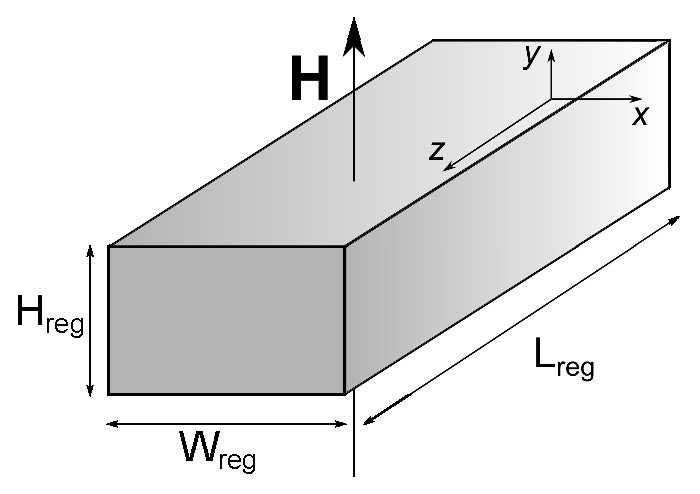
\includegraphics[width=8cm]{Fig1-reg3d}
  \caption{AMR model geometry}
  \label{fig:amrmodel}
\end{figure}

\nomenclature[ah]{$H\ped{reg}$}{regenerator height [\si{\meter}]}
\nomenclature[aw]{$W\ped{reg}$}{regenerator width [\si{\meter}]}
\nomenclature[al]{$L\ped{reg}$}{regenerator length [\si{\meter}]}
\nomenclature[ah]{$H$}{magnetic field [\si{\henry}]}

The momentum equation for the fluid domain is given by:

\begin{equation}
\label{eq:75}
  \frac{\rho\ped{f}}{\varepsilon} \diffp{V_z}{t}= -\diffp{P}{z} - \frac{\mu\ped{f}}{K} V_z - \frac{c\ped{E} \rho\ped{f}}{K^{1/2}} \left| V_z\right| V_z 
\end{equation}

\nomenclature[ak]{$K$}{permeability of the porous medium [\si{\meter\squared}]}
\nomenclature[ac]{$c\ped{E}$}{Ergun constant of the porous medium}
\nomenclature[br]{$\rho$}{density [\si{\kg\per\cubic\meter}]}
\nomenclature[be]{$\varepsilon$}{porosity}
\nomenclature[av]{$V$}{velocity [\si{\meter\per\second}]}
\nomenclature[ap]{$P$}{pressure [\si{\pascal}]}
\nomenclature[bu]{$\mu\ped{f}$}{fluid dynamic viscosity [\si{\pascal\second}]}


\noindent where the macroscopic inertial term on the left-hand side is balanced with the pressure gradient, Darcy stress and Forchheimer drag \cite{bib:nield06_convec_porous_media}. The momentum equation is solved for the time-dependent uniform fluid velocity $V_z$ through the bed. 

The energy equation for the fluid phase can be written as:

\begin{equation}
\label{eq:78}
\begin{split}
  \rho\ped{f} c_{p,\mathrm{f}} \left(\varepsilon \diffp{T\ped{f}}{t} + V_z\diffp{T\ped{f}}{z}\right) = & -\hheat\ped{sf} \beta \left(T\ped{f} - T\ped{s}\right) \\
& + \left|V_z\diffp{P}{z}\bigg|_f \right| \\
& + \varepsilon\left(k\ped{f}\ap{eff}  +\rho\ped{f} c_{p,\mathrm{f}} D\ped{ld}\right)\diffp[2]{T\ped{f}}{z} \\
& + \rate{q}\ped{csg}  
\end{split}
\end{equation}

\noindent where the left-hand side includes the inertial and advection terms, and the right-hand side includes terms for the solid-fluid heat transfer, viscous dissipation, heat conduction, porous-media dispersion, and casing losses.

\nomenclature[at]{$T$}{temperature [\si{\kelvin}]}
\nomenclature[at]{$t$}{time [\si{\second}]}
\nomenclature[ax]{$x,y,z$}{coordinate system variables [\si{\meter}]}
\nomenclature[ip]{$p$}{constant-pressure}

\nomenclature[aq]{$\rate{q}\ped{csg}$}{volumetric casing losses in the AMR model [\si{\watt\per\cubic\meter}]}
\nomenclature[ic]{csg}{regenerator casing}
\nomenclature[ah]{$\hheat$}{heat transfer coefficient [\si{\watt\per\meter\squared\per\kelvin}]}
\nomenclature[aa]{$A\ped{sf}$}{contact surface area between solid and fluid phases in the regenerator [\si{\meter^2}]}
\nomenclature[is]{sf}{relative to the heat transfer between solid and fluid phases in the regenerator}
\nomenclature[bb]{$\beta$}{surface area density [\si{\square\meter\per\cubic\meter}]}
\nomenclature[ak]{$k$}{thermal conductivity [\si{\watt\per\meter\per\kelvin}]}
\nomenclature[ad]{$D\ped{ld}$}{dispersion term in the AMR model [\si{\meter\square\per\second}]}
\nomenclature[af]{$f$}{cycle frequency [\si{\hertz}]}
\nomenclature[am]{$m$}{mass [\si{\kg}]}

\nomenclature[bt]{$\tau$}{time period [\si{\second}]}
\nomenclature[ac]{$c$}{specific heat [\si{\joule\per\kg\per\kelvin}]}


The energy equation for the solid phase is written as:

\begin{equation}
\label{eq:88}
  \rho\ped{s} c\ped{s}(1 - \varepsilon)\diffp{T\ped{s}}{t} = \hheat\ped{sf}\beta(T\ped{f}-T\ped{s}) + (1-\varepsilon)k\ped{s}\ap{eff}\diffp[2]{T\ped{s}}{z}
\end{equation}

\noindent where the terms represent respectively inertia, solid-fluid heat transfer and heat conduction.

Initial and boundary conditions, closure relations for the porous media terms, solution methods and convergence criteria and analyses are discussed in detail in \cite{bib:trevizoli16_perfor_model}. This AMR model solves the above equations for one regenerator operating between given sources temperatures (assuming ideal heat exchangers in contact with the thermal reservoirs), during one full cycle (hot and cold blows and  magnetization and demagnetization periods), given specified operating conditions (to be discussed later).

The casing heat transfer term $\rate{q}\ped{csg}$ in \autoref{eq:78} is calculated solving the heat conduction equation in the regenerator casing \cite{bib:trevizoli16_perfor_model}. It can be neglected in some circumstances if an insulating casing material is assumed, which greatly simplifies the analysis. 

\subsubsection{Fluid flow profile modeling}
\label{sec:how-fluid-flow}

The pressure gradient in \autoref{eq:75} is modeled as:

\begin{equation}
\label{eq:76}
-\diffp{P}{z} = \rho\ped{f} A\ped{t} g(t)
\end{equation}

\noindent where \(g(t)\) is a dimensionless function that expresses the mathematical waveform of the pressure gradient, and  \(A\ped{t}\) is its amplitude,  adjusted in a convergence loop. In this loop, the mass flow rate calculated in term of the Darcy velocity from \autoref{eq:75} is compared with the input   mass flow rate until convergence is obtained. 

\nomenclature[ag]{$g(t)$}{dimensional waveform of the pressure gradient term in the fluid momentum equation}
\nomenclature[aA]{$A\ped{t}$}{amplitude of the pressure gradient waveform in the fluid momentum equation [\si{\meter\per\second\squared}]}

The canonical fluid flow profile considered in this work is the square wave or \emph{instantaneous profile}, because of the instantaneous change in flow rate, as shown in \autoref{fig:mprofile}. 

\begin{figure}[!ht]
  \centering
  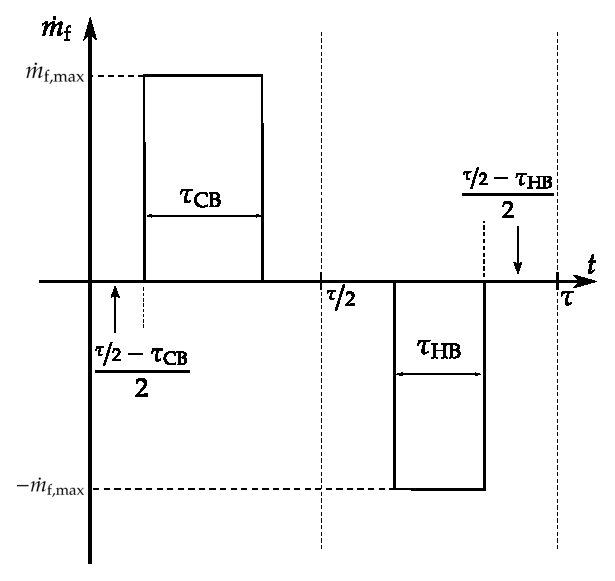
\includegraphics[width=8cm]{Fig2-mprofile}
  \caption{Instantaneous fluid flow profile. Adapated from \cite{bib:fortkamp20-desig}.}
  \label{fig:mprofile}
\end{figure}

The instantaneous mass flow rate, \(\rate{m}\ped{f}(t)\), is defined over a cycle with a period \(\tau\), and represents the fluid flow through a given regenerator bed. The so-called \emph{hot cycle}, during which the MCM is magnetized, occupies the time interval \(0 \le t < \nicefrac{\tau}{2}\), while the \emph{cold cycle} lies between \(\nicefrac{\tau}{2} \le t \le \tau\). The flow profile oscillates between two plateaus of equal magnitude
\(\rate{m}\ped{f,max}\) and opposite directions, which are centered in each half-cycle. During the hot cycle, the cold
blow period is \(\tau\ped{CB}\), and during the cold cycle the hot blow period is \(\tau\ped{HB}\). If balanced flow exists, then \(\tau\ped{CB} = \tau\ped{HB}\).


During each half cycle, there are periods without  fluid flow defined as:

\begin{equation}
\label{eq:48}
\tau\ped{0,HC} = \frac{\nicefrac{\tau}{2} - \tau\ped{CB}}{2}
\end{equation}

\begin{equation}
\label{eq:49}
\tau\ped{0,CC} = \frac{\nicefrac{\tau}{2} - \tau\ped{HB}}{2}
\end{equation}

where HC and CC stand for hot cycle and cold cycle, respectively.

\nomenclature[vh]{HC}{hot cycle}
\nomenclature[vc]{CC}{cold cycle}
\nomenclature[vc]{CB}{cold blow}
\nomenclature[bt]{$\tau\ped{0,CC}, \tau\ped{0,HC}$  }{time periods without fluid flow in the respective half-cycle (see list of Abbreviations) [\si{\second}]}

The profile can be mathematically defined as:

\begin{equation}
\rate{m}\ped{f}(t)=
\begin{cases}
0, & 0 \le t < \tau\ped{0,HC} \\
\rate{m}\ped{f,max}, & \tau\ped{0,HC} \le t \le \nicefrac{\tau}{2} - \tau\ped{0,HC} \\
0, & \nicefrac{\tau}{2} - \tau\ped{0,HC} < t < \nicefrac{\tau}{2} + \tau\ped{0,CC} \\
-\rate{m}\ped{f,max}, & \nicefrac{\tau}{2} + \tau\ped{0,CC} \le t \le \tau - \tau\ped{0,CC} \\
0, &  \tau - \tau\ped{0,CC} <  t < \tau \\
\end{cases}
\label{eq:50}
\end{equation}

When the blows have different time durations, the AMR cycle is considered unbalanced, and that is known to have a negative effect on performance \cite{bib:eriksen16_effec,bib:nakashima18-influen-exp}. In this work, the blows are always balanced, hence the blow fraction, i.e., the ratio of blow durations to cycle period \cite{bib:nakashima18-influen-exp}, can be evaluated as:

\begin{equation}
\label{eq:59}
F\ped{B} = \frac{2\tau\ped{B}}{\tau}
\end{equation}

\noindent where $\tau\ped{B}$ is the duration of one blow.

\nomenclature[bt]{$\tau\ped{B}$}{blow duration [\si{\second}]}
\nomenclature[af]{$F\ped{B}$}{blow fraction}

\subsubsection{Magnetic profile modeling}
\label{sec:how-magnetic-profile}

The magnetic profile is modeled by a waveform of magnetic field strength, $H(t)$, applied perpendicular to the regenerators, as shown in \autoref{fig:amrmodel}. The magnetic field is assumed uniform throughout the beds. The applied field is corrected from demagnetization effects to yield the effective field inside the regenerators:

\begin{equation}
  \label{eq:6}
  H\ap{eff} = H - N\ped{D} M
\end{equation}

\nomenclature[am]{$M$}{magnetization field [\si{\henry}]}
\nomenclature[an]{$N\ped{D}$}{demagnetization tensor}
\nomenclature[ie]{eff}{effective}

\noindent where $M$ is the magnetization field of the material, and $N\ped{D}$ is a demagnetization factor.

The magnetocaloric effect is implemented in the so-called discrete approach \cite{bib:nielsen11_review}; every time the magnetic field changes, based on the input magnetic profile, the solid temperature is calculated according to:

\begin{equation}
  \label{eq:89}
  T\ped{s}(t + \Delta{}t) = T\ped{s}(t) + \dtad \left(T\ped{s}(t),H\ap{eff}(t),H\ap{eff}\left(t + \Delta{}t\right)\right)
\end{equation}


\nomenclature[at]{$\dtad$}{adiabatic temperature variation [\si{\kelvin}]}

\noindent where the adiabatic temperature variation, $\dtad$, a standard measure of the MCE, is calculated from tabulated experimental data for magnetocaloric materials as function of temperature and effective field. \cite{bib:trevizoli16_perfor_model}. Experimental curves of $\dtad$ can be found in \cite{bib:bahl09}.

The magnetic profiles considered in this work are presented in terms of the flux density $B = \mu_0 H$, where $\mu_0$ is the permeability of free space; the magnetic field $H$ is used in the evaluation of the magnetocaloric effect (cf. Sec.~\ref{sec:how-magnetic-profile}).

\nomenclature[ab]{$B$}{magnetic flux density [\si{\tesla}]}
\nomenclature[bu]{$\mu_0$}{magnetic permeability of free space [\si{\henry\per\meter}]}


The instantaneous (square wave) profile (represented by the subscript ``IT'') and the rectified cosine profile (represented by ``RC'') are defined solely in terms of the extreme values $B\ped{min}$ and $B\ped{min}$, and are shown in \autoref{fig:itrc}.

\nomenclature[vi]{IT}{instantaneous magnetic profile}
\nomenclature[vr]{RC}{rectified cosine magnetic profile}

\begin{equation}
{B}\ped{IT}\,(t)=
\begin{cases}
{B}\ped{max}, & 0 \le t < \nicefrac{\tau}{2} \\
{B}\ped{min}, & \nicefrac{\tau}{2} \le t < \tau\\
\end{cases}
\label{eq:199}
\end{equation}

\begin{equation}
{B}\ped{RC}\,(t) = B\ped{min} + \left(B\ped{max} - B\ped{min}\right)  \left\lvert \cos\left( \frac{\pi}{\tau} \left( t - \frac{\tau}{4}\right)\right) \right\rvert
\label{eq:200}
\end{equation}

\begin{figure}[!ht]
  \centering
  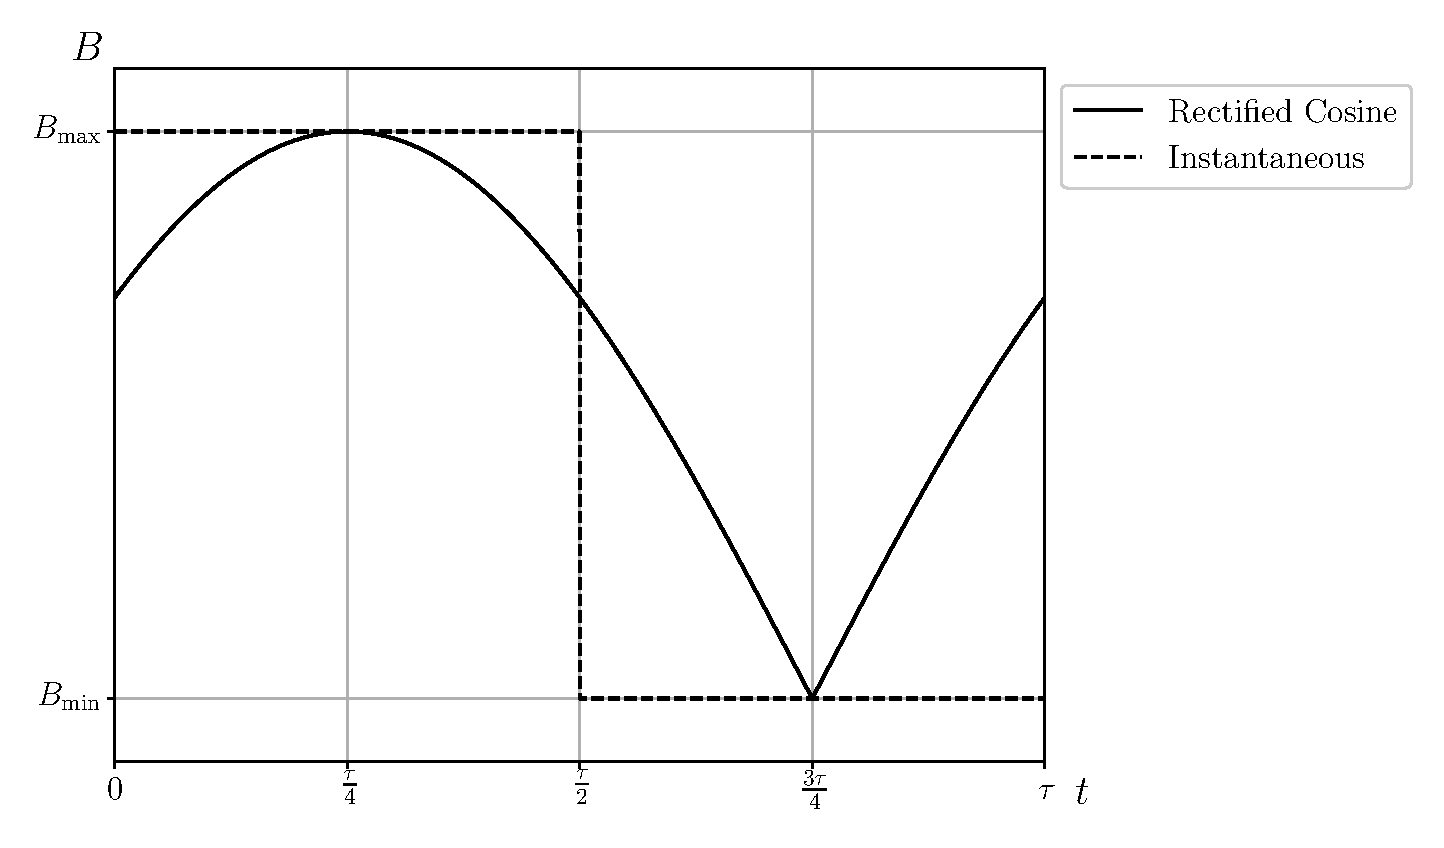
\includegraphics[width=8cm]{Fig3-profiles_it_and_rc}
  \caption{Instantaneous ("IT") and rectified cosine ("RC") magnetic profiles}
  \label{fig:itrc}
\end{figure}

A suitable approximation of the instantaneous profile is the \emph{magnetic ramp profile}, shown in \autoref{fig:ramp}, with finite transition times between the levels of constant magnetization. The magnetic profile oscillates  between a low value \({B}\ped{min}\) and a high value \({B}\ped{max}\), and remains at each plateau for a period of \(\tau\ped{M}\). The plateaus are balanced and centered at each half-cycle.

\begin{figure}[!ht]
  \centering
  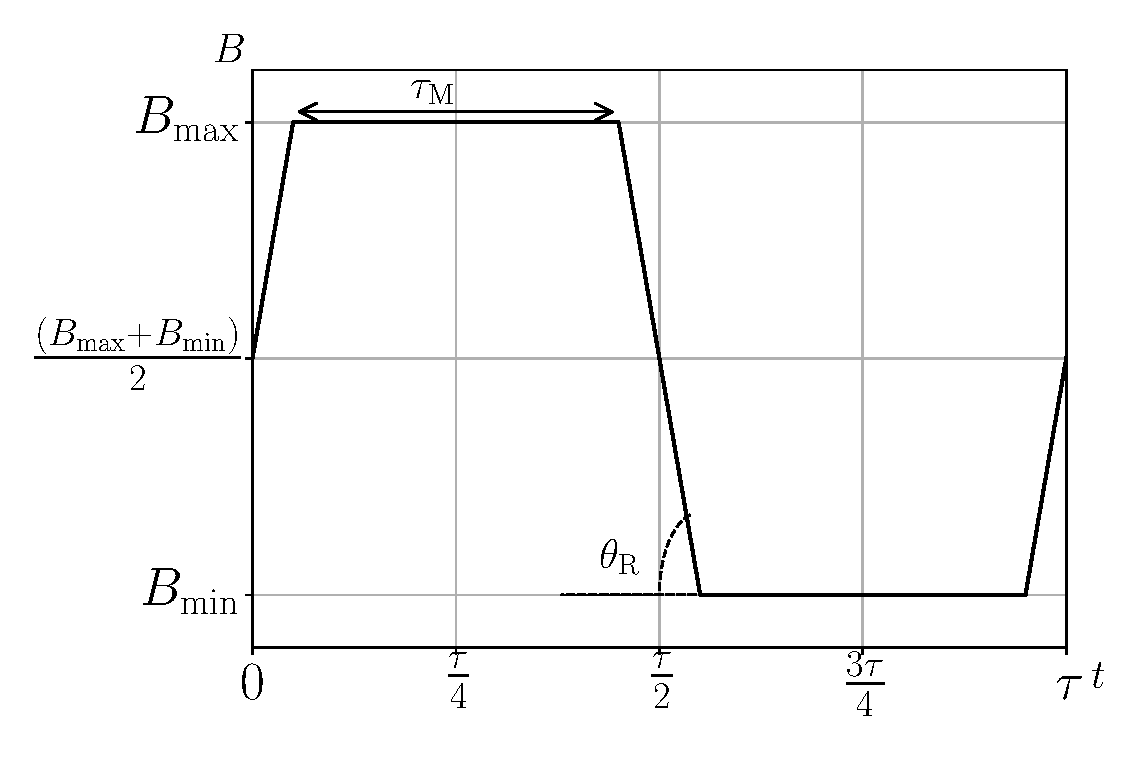
\includegraphics[width=7cm]{Fig4-profile_rm}
  \caption{\textcolor{black}{Magnetic ramp}  profile}
  \label{fig:ramp}
\end{figure}

The \emph{ramp period} \(\tau\ped{R}\) is defined as:

\begin{equation}
\label{eq:201}
\tau\ped{R} = \frac{1}{4}\left(\tau - 2 \tau\ped{M}\right)
\end{equation}

\noindent such that there are four ramp periods in one full cycle. The ramp rate, \(\tan \theta\ped{R}\), is:

\begin{equation}
\label{eq:202}
\tan \theta\ped{R} = \frac{\left({B}\ped{max} - {B}\ped{min}\right)}{2\tau\ped{R}}
\end{equation}

\nomenclature[bt]{$\tau\ped{R}$}{ramp period in the magnetic ramp profile [\si{\second}]}
\nomenclature[bt]{$\tau\ped{M}$}{magnetization period in the magnetic ramp  profile [\si{\second}]}
\nomenclature[bo]{$\tan \theta\ped{R}$}{ramp rate in the magnetic ramp profile [\si{\tesla\per\second}]}

The magnetization fraction, \(F\ped{M}\), is the fraction of the cycle during which the magnetocaloric material is subjected to a constant magnetic field:

\begin{equation}
\label{eq:204}
F\ped{M} = \frac{2\tau\ped{M}}{\tau}
\end{equation}

\nomenclature[af]{$F\ped{M}$}{magnetization fraction}

The ramp profile (``RM'') can be mathematically defined as:

\begin{equation}
{B}\ped{RM}(t)=
\begin{cases}
\nicefrac{\left({B}\ped{max} + {B}\ped{min}\right)}{2} + t \tan \theta\ped{R} , & 0 \le t < \tau\ped{R} \\
{B}\ped{max}, & \tau\ped{R} \le t < \nicefrac{\tau}{2} - \tau\ped{R}\\
{B}\ped{max} - \left(t - \left(\nicefrac{\tau}{2} - \tau\ped{R}\right)\right) \tan \theta\ped{R} , & \nicefrac{\tau}{2} - \tau\ped{R} \le t < \nicefrac{\tau}{2} + \tau\ped{R} \\
{B}\ped{min}, & \nicefrac{\tau}{2} + \tau\ped{R} \le t < \tau - \tau\ped{R}\\
{B}\ped{min} + \left(t - \left(\tau - \tau\ped{R}\right)\right) \tan \theta\ped{R} , & \tau - \tau\ped{R} \le t \le \tau \\
\end{cases}
\label{eq:203}
\end{equation}

\nomenclature[vr]{RM}{ramp magnetic profile}

Additionally, the average values of the magnetic field during each half-AMR cycle are considered for comparison between profiles. The average magnetic profile during the hot cycle ($0 \le t < \nicefrac{\tau}{2}$) is denoted by $\average{B}\ped{high}$ and the average during the cold cycle  ($ \nicefrac{\tau}{2} \le t < \tau$) is denoted by $\average{B}\ped{low}$. For the instantaneous waveform, these average values are identical to the extreme values.

\subsubsection{Evaluation of solid and fluid properties}
\label{sec:eval-solid-fluid}

The fluid properties are considered constant in the momentum equation to decouple the solution procedures to determine the velocity and temperature fields. The properties are computed at the average temperature between the hot and cold sources, and are evaluated from interpolation of tables imported from the EES software \cite{bib:klein13-ees}. In all simulations shown in this work, the heat transfer fluid is a \num{80}/\SI{20}{\percent} vol.~mixture of water/ethylene-glycol. For the energy equations, the fluid properties are also calculated from tabulated data, but the temperature dependence is considered.


Both single- and multilayer regenerators are considered in this study. Single-layer regenerators are composed of gadolinium,  a benchmark material with a Curie temperature of \SI{290}{\kelvin}. For simplicity, the solid density is assumed constant at $\rho\ped{s} = \SI{7900}{\kg\per\cubic\meter}$ and the solid thermal conductivity is set to $k\ped{s} = \SI{10.5}{\watt\per\meter\per\kelvin}$. The specific heat capacity of \ce{Gd} is calculated as a function of temperature and magnetic field based on experimental data, using a bi-linear interpolation scheme; more details on the experimental dataset are available in \cite{bib:trevizoli16_perfor_model}. 

For the multilayer simulations, alloys of gadolinium and yttrium are used in the form \ce{Gd_{1-x}Y_x}, where $x$ is the yttrium fraction.  This fraction reduces the Curie temperature of the alloy relative to that of pure gadolinium. Due to the lack of experimental  data on the magnetocaloric properties of \ce{Gd_{1-x}Y_x} alloys at the time this analysis was made, a simpler approach was used in which the dependence of magnetization, specific heat capacity and entropy with respect to the magnetic field for alloys with a low yttrium fraction are identical to those of pure gadolinium, but are shifted to a lower Curie temperature (corresponding to the yttrium fraction). 

\nomenclature[ix]{$x$}{yttrium fraction}

\subsubsection{Performance metrics}
\label{sec:performance-metrics}

The AMR model is solved for only one bed, but  assumes that the $N\ped{reg}$ identical beds experience the same cycle. Thus, the extensive performance parameters are multiplied by that factor.

\nomenclature[an]{$N\ped{reg}$}{number of regenerators}

The cooling capacity is calculated as \cite{bib:trevizoli16_perfor_model}:

\begin{equation}
\label{eq:99}
\qc = N\ped{reg}\frac{1}{\tau} \int_{\tau\ped{HB}} \mrate\ped{f}(t) c_{p,\mathrm{f}} \left( T\ped{C} -T\ped{f,CE} \right) \diffd{t}
\end{equation}


\nomenclature[vh]{HB}{hot blow}
\nomenclature[vc]{CE}{cold end}
\nomenclature[am]{$\mrate\ped{f}$}{mass flow rate [\si{\kg\per\second}]}
\nomenclature[vc]{C}{cold source}
\nomenclature[vc]{H}{hot source}
\nomenclature[aq]{$\qc$}{cooling capacity [\si{\watt}]}


As pointed out in \cite{bib:fortkamp20-desig}, since external sources of irreversibility (e.g., heat transfer with a finite temperature difference in the heat exchangers) are ignored and no eddy currents and hysteresis losses are present, the magnetic power required to magnetize the solid refrigerant and produce the MCE in the AMR cycle is given by the product of the Carnot efficiency and the cooling capacity as follows:

\begin{equation}
\label{eq:100}
\wmag = \qc \frac{T\ped{H} - \tc}{\tc}
\end{equation}

Irreversibility due to fluid friction is accounted for in the calculation of the pumping power:

\begin{equation}
\label{eq:103}
\wpump = N\ped{reg}\frac{1}{\tau}\int_0^{\tau}\frac{\rate{m}\ped{f}}{\rho\ped{f}} \Delta P \diffd{t}
\end{equation}

\noindent where $\Delta P$ is the total pressure drop through the regenerator (including one hot and one cold blow).

\nomenclature[awm]{$\wpump$}{pumping power [\si{\watt}]}
\nomenclature[awm]{$\wmag$}{magnetic power [\si{\watt}]}
\nomenclature[ap]{$\Delta P$}{total pressure drop across one regenerator [\si{\pascal}]}

\subsection{Hydraulic system  and fluid flow profile model}
\label{sec:hydr-syst-model}


The hydraulic system designed to modulate the fluid flow through different regenerators at different time instants is composed of a pump and a set of electronic valves which can be precisely controlled to yield the desired blow durations. The electrical power consumed by the valve array is computed separately from other work contributions.

% Type R = Type B (BuRkert)
% Type S = Type A (ASco)

In the present analysis, two types of valves are considered. In the first approach, called \emph{Type R valves}, the  model proposed in \cite{bib:cardoso16_trans} is used, assuming that the individual consumption of each valve is independent of frequency and blow fraction. The valve power  $\wvalve$ can be computed as:


\begin{equation}
  \label{eq:58}
  \wvalve = N\ped{v}F\ped{B}\left(\wvalven + \frac{1}{2}\wrelayn\right)
\end{equation}

\noindent where $N\ped{valve}$ is the number of valves, $\wvalven$ is the measured average nominal power for one normally-closed electronic valve and $\wrelayn$ is the nominal power for one controlling relay. The factor $\nicefrac{1}{2}$ is due to two valves being controlled by one relay.

\nomenclature[an]{$N\ped{valve}$}{number of valves}
\nomenclature[aw]{$\wvalve$}{valve power [\si{\watt}]}
\nomenclature[aw]{$\wvalven$}{nominal power comsumption of one valve [\si{\watt}]}
\nomenclature[aw]{$\wrelayn$}{nominal power comsumption of one relay [\si{\watt}]}

In the second approach, \emph{Type S} valves are used, with  nominal power lower in magnitude but which depends on frequency and blow fraction. These valves were experimentally characterized by \cite{bib:cardoso18}, where a single valve was attached to a measurement circuit and set to operate for varying values of blow fraction and frequency; the valve power was calculated from the averaged values of voltage and current after periodic steady state was reached. From these experiments, the valve power was experimentally correlated as:

\begin{equation}
  \label{eq:198}
  \wvalve\,[\si{\watt}]= N\ped{valve}\left(0.927 f\,[\si{\hertz}] + 1.023 F\ped{B} + 0.226 f\,[\si{\hertz}] F\ped{B} - 0.037\right)
\end{equation}

Equation~\eqref{eq:198} was correlated for blow fractions of \num{50} and \SI{100}{\percent} and frequencies in the range of \num{0.2}--\SI{1.6}{\hertz}, with an uncertainty on the order of \SI{0.4}{\watt} for a single valve. The use of different valve types will be discussed among the presented results.

Independent of the valve type used, it is also assumed that each valve system can produce the fluid flow profile shown in \autoref{fig:mprofile}, where the displaced fluid mass during one blow in one regenerator bed is $\rate{m}\ped{f,max} F\ped{B} \nicefrac{\tau}{2}$. The \emph{utilization factor} can then be calculated as:

\begin{equation}
  \label{eq:110}
  \Phi = \frac{\rate{m}\ped{f,max} F\ped{B} c\ped{f}}{2 f m\ped{s} c\ped{s}}
\end{equation}

\nomenclature[bf]{$\Phi$}{utilization factor}
\noindent and in all results shown in this work, the number of valves is calculated as:

\begin{equation}
  \label{eq:111}
  N\ped{valve} = 2 N\ped{reg}
\end{equation}

\subsection{Calculation of the coefficient of performance}
\label{sec:calc-coeff-perf}

The coefficient of performance takes the cooling capacity as the main output parameter from the AMR model, in addition to all previously cited power contributions:

\begin{equation}
  \label{eq:112}
  \cop = \frac{\qc}{\wpump + \wmag + \wvalve}
\end{equation}



\section{Results and Discussions}
\label{sec:results-discussions}

The analysis of magnetic profiles was performed at two different stages. Initially, the instantaneous (square-wave) and the rectified cosine profiles are compared using a simpler approach (i.e., neglecting casing losses). Later, based on the selection of the most promising magnetic profile, a more in-depth analysis is carried out to determine the optimal geometric and operating parameters of the AMR system.

\subsection{Comparison of instantaneous and rectified cosine profiles using a simplified model}
\label{sec:comp-cosine-inst}

At the first stage of the present analysis, the instantaneous and rectified cosine profiles are compared considering a single-layer regenerator  without casing losses, using Type R valves. The parameters used in all simulations are presented in \autoref{tab:params-cobem}.

\begin{table}[!ht]
  \centering
  \caption{AMR parameters kept fixed in the simulations with different magnetic profiles}
  \begin{tabular}{c|c}
\hline
\textbf{Parameter} & \textbf{Value}\\
\hline
   $D\ped{p}$ & \SI{0.5}{\mm}\\
$H\ped{reg}$ & \SI{20}{\mm}\\
$W\ped{reg}$ & \SI{25}{\mm}\\
$L\ped{reg}$ & \SI{100}{\mm}\\
$N\ped{reg}$ & 11 \\
$N\ped{valve}$ & 22 \\
$T\ped{H}$ & \SI{298}{\kelvin}\\
$\tc$ & \SI{278}{\kelvin}\\
$\wvalven$ & \SI{4}{\watt}\\
$\wrelayn$ & \SI{0.36}{\watt}\\
\hline
  \end{tabular}

  \label{tab:params-cobem}
\end{table}

\nomenclature[ad]{$D\ped{p}$}{particle diameter [\si{\meter}]}


When comparing the performances resulting from the application of the different magnetic profiles, the same average magnetic field during the hot cycle will be considered; this implies a higher peak for the rectified cosine. For the cold cycle, the minimum values for both profiles are the same, as shown in \autoref{fig:comparison-methods-profiles}. For reference, in all simulations,  the minimum value for the rectified cosine was fixed at ${B}\ped{min} = \SI{0.1}{\tesla}$. 

\begin{figure}[!ht]
  \centering
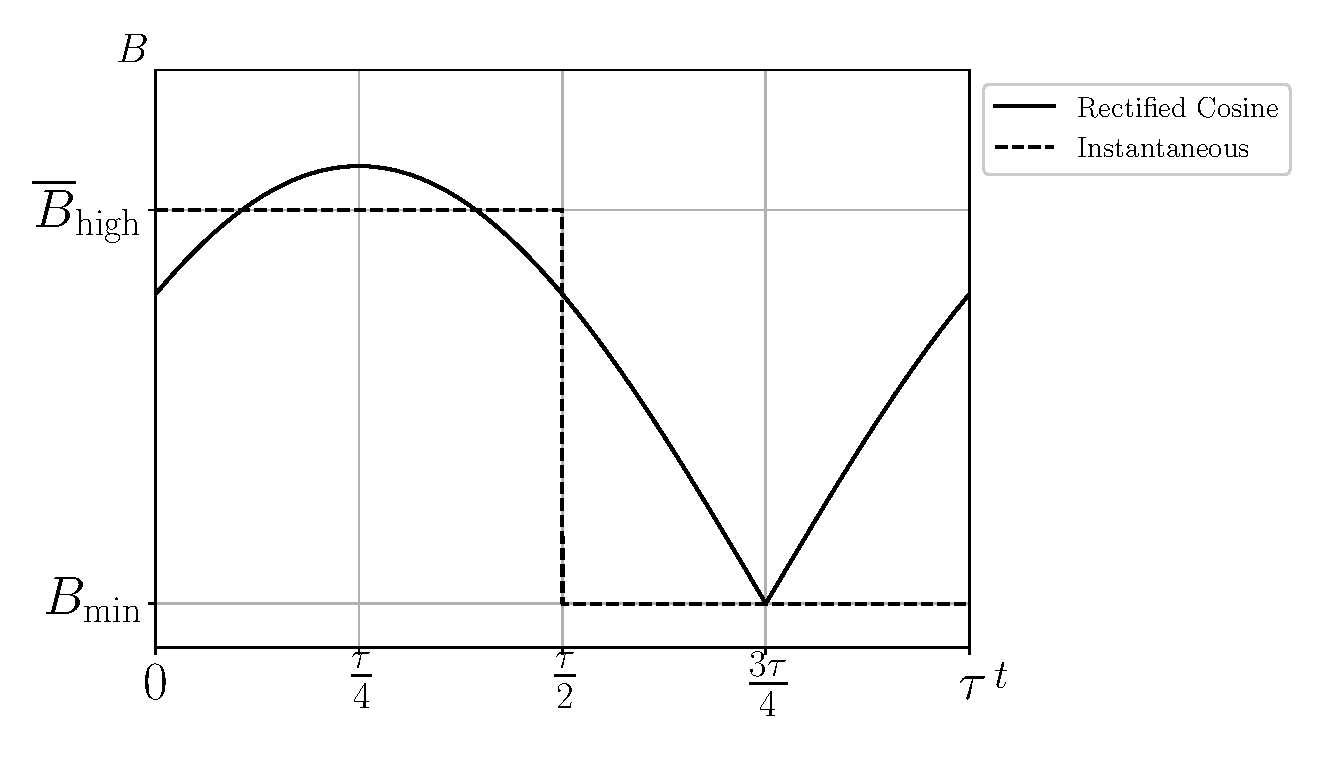
\includegraphics[width=8cm]{Fig5-profiles_it_and_rc_same_minimum}
  \caption{Configuration of average and extreme values of the instantaneous and rectified cosine profiles }
  \label{fig:comparison-methods-profiles}
\end{figure}

Simulations were carried out for various values of blow fraction. The rectified cosine profile can benefit from a smaller blow fractions that concentrate the flow during the periods of very high and very low fields, thereby increasing the average variation in magnetic field \cite{bib:nakashima18-influen-exp}; this does not happen with the instantaneous profile, since the field is constant and reducing the blow fraction will only reduce the period where the fluid is in contact with the warmed up solid, decreasing the regenerator effectiveness. In this section, all results use the critical value of blow fraction that maximized the cooling capacity: fluid flowing during the entire period for the instantaneous profile, and only during \SI{60}{\percent} of the period (the smallest blow fraction tested) for the cosine profile; this latter case is shown in \autoref{fig:cos-inst-60}.

\begin{figure}[!ht]
  \centering
  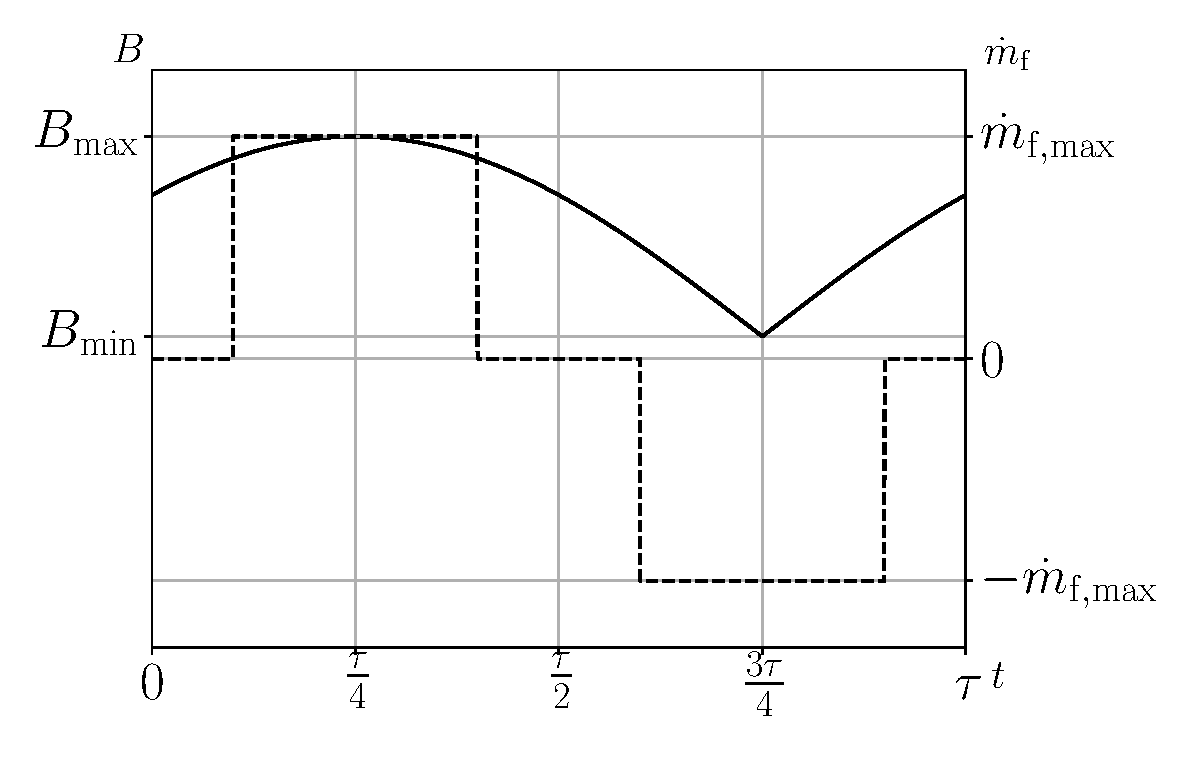
\includegraphics[width=7cm]{Fig6-profiles_rc_and_flow_instantaneous}
  \caption{Rectified cosine magnetic profile (solid lines) and the instantaneous flow profile  with blow fraction of \SI{60}{\percent} (dashed lines)}
  \label{fig:cos-inst-60}
\end{figure}

Figure~\ref{fig:cos_ins} shows the cooling capacity attained by the device at a frequency of \SI{1}{\hertz} and different utilizations. The horizontal axis shows the average field value during the high field region. The instantaneous profile almost always yields a higher performance, and since the average field during the hot cycle (high field stage) is the same, the main difference is due to the low magnetic field levels. In this comparison, the instantaneous profile is capable of keeping a low magnetic field over the entire half-cycle, which is beneficial for performance; as demonstrated by \cite{bib:asme-mce}, a higher average magnetic field during the low-field stage increases the solid temperature and consequently results in  warmer fluid entering the cold heat exchanger, representing a thermal loss. Analyzing points of different profiles of constant utilization (which should result in the same regenerator effectiveness), 
 for $\Phi=1.0$ and $B\ped{high} = \SI{1.40}{\tesla}$, the cooling capacity for the instantaneous profile is $\SI{196.3}{\percent}$ higher than for the cosine profile. This is the result of the fluid being able to cool down to lower temperatures during the low-field cycle, since the cosine profile cannot maintain the field as low as the instantaneous profile (cf. \autoref{fig:comparison-methods-profiles}), even with the reduction of blow fraction.


\begin{figure}[!ht]
  \centering
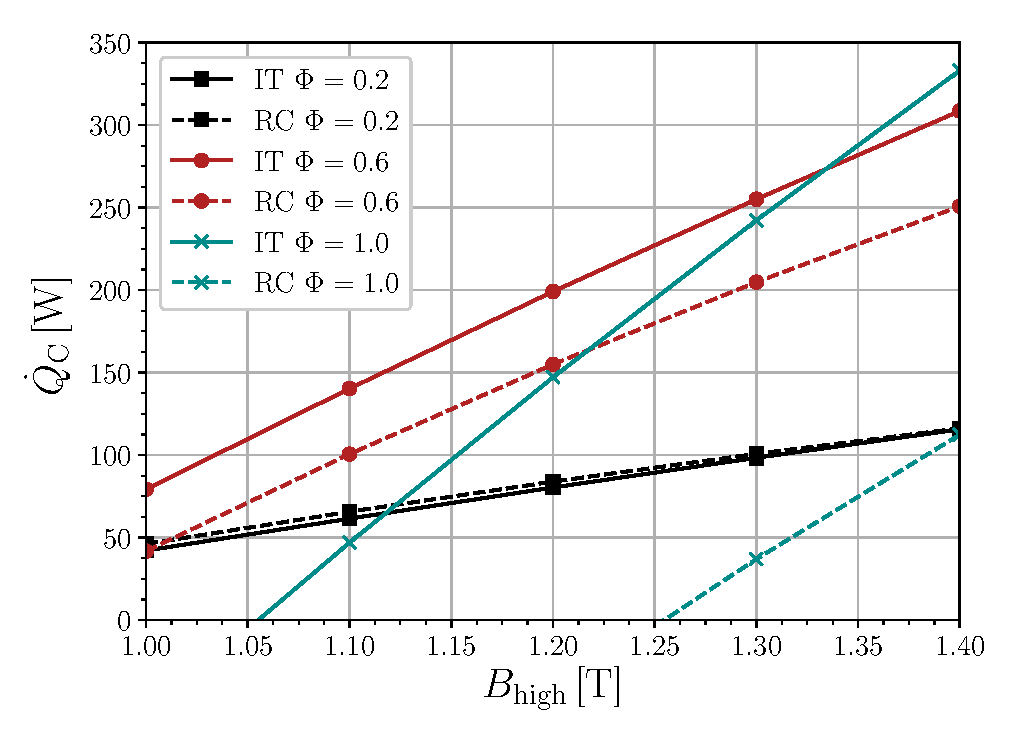
\includegraphics[width=8cm]{Fig7-Qc_B_comp_f_1_same_minimum}
  \caption{Cooling capacity as a function of the  average high magnetic field, for different utilizations. \textcolor{black}{``IT''}: instantaneous (blow fraction of \SI{100}{\percent}); ``RC'': rectified cosine  (blow fraction of \SI{60}{\percent}).}
 \label{fig:cos_ins}
\end{figure}

The only exception in this comparison is observed for the lowest utilization of $\Phi = 0.2$, where the performance is slightly better for the RC profile. Since the blow fraction for the cosine is smaller, the mass flow rate is higher in the latter for the same utilization (cf. Eq.~\eqref{eq:200}). This increases the heat transfer rate, as previously explained ---  outweighing the effects of the magnetic field.

Also noticeable in \autoref{fig:cos_ins} is the non-linear relationship  between cooling capacity and utilization. For instance, for the ``RC'' profile at the highest magnetic field, the cooling capacity increases when the utilization grows from 0.2 to 0.6, but then return to the same levels with a further increase of utilization to 1.0. Since the frequency is constant for \autoref{fig:cos_ins}, increasing utilization means increasing the mass flow rate; initially, this results in higher heat transfer rates due to higher Nusselt numbers, but further increase reduce the effectiveness and amplify viscous dissipation, to the point where the cooling capacity is null for certain points with the highest utilization. 

The same analysis, but in terms of the coefficient of performance, is shown in \autoref{fig:cos_ins_cop}, where  the instantaneous profile yields better results for medium to high levels of utilization. This is explained by the behavior of the magnetic, valve and pumping power shown in   \autoref{fig:cos_ins_w} for a fixed utilization of 0.6. As can be seen, the magnetic power only differs between the profiles due to changes in cooling capacity. Also, the valve power is higher for the instantaneous profile since the valves must remain open for longer periods. However, the proportional increase in pumping power, due to arger larger flow rates, is even higher (than the change in valve power).

\begin{figure}[!ht]
  \centering
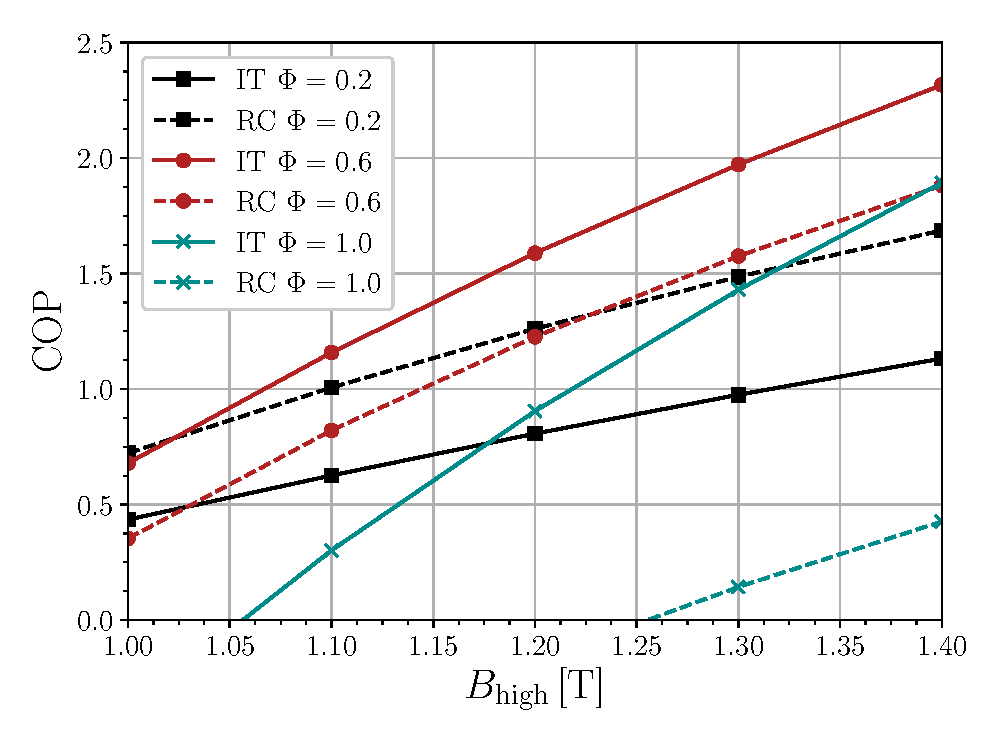
\includegraphics[width=7cm]{Fig8-COP_B_comp_f_1_same_minimum}
  \caption{Coefficient of performance as a function of the  average high magnetic field, for different values of utilization. ``IT'': instantaneous (blow fraction of \SI{100}{\percent}); ``RC'': rectified cosine  (blow fraction of \SI{60}{\percent}).}
 \label{fig:cos_ins_cop}
\end{figure}



\begin{figure}[!ht]
  \centering
  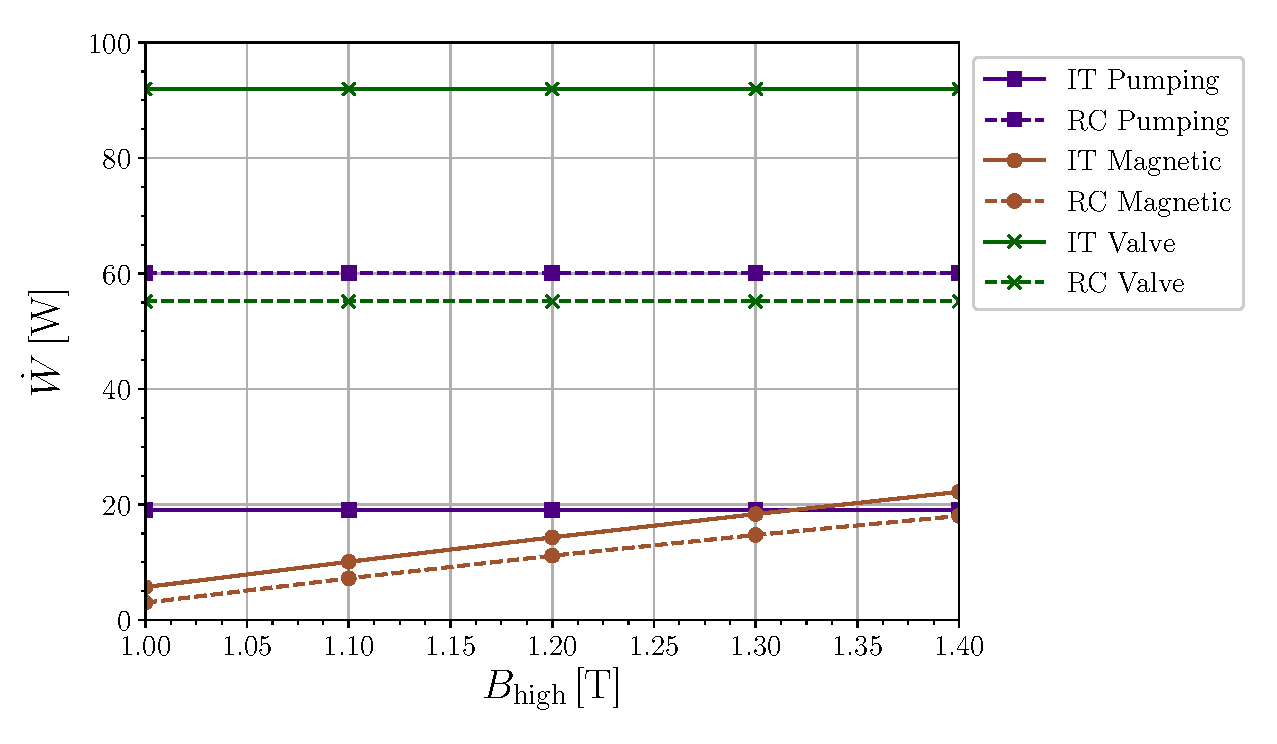
\includegraphics[width=10cm]{Fig9-W_B_comp_f_1_Phi_60_same_minimum}
  \caption{Power contributions as functions of the average high magnetic field, for a utilization of 0.6. ``IT'': instantaneous (blow fraction of \SI{100}{\percent}); ``RC'': rectified cosine  (blow fraction of \SI{60}{\percent}).}
  \label{fig:cos_ins_w}
\end{figure}

In general, considering target values for the cooling capacity, AMRs operating with the instantaneous magnetic profile lead to better performance results. As can be seen in Fig.~\ref{fig:cos_ins}, an instantaneous profile with the lowest possible value of $B\ped{min}$ and the highest possible value of $B\ped{max}$, with a flow profile occupying the whole cycle with average values of utilization, results in the highest values of cooling capacity among all simulations. 

The rectified cosine profile, found in compact systems using Halbach arrays, can surely benefit from reducing the blow fraction, both in terms of cooling capacity and temperature span. However, for the typical parameters evaluated in this paper, even if the blow fraction is optimized for the ``RC'' profile, the ``IT'' profile still gives better results.

\subsubsection{Analysis of the instantaneous profile}
\label{sec:deta-analys-inst}

As shown in the previous section, the instantaneous profile generally yields the highest values of cooling capacity. Therefore, in this section, a more detailed analysis of this profile is carried out, where the maximum field is varied, but the minimum value is kept at \SI{0.05}{\tesla}. Figure~\ref{fig:qc_phi_inst} shows the cooling capacity as a function of the utilization, for several levels of the maximum magnetic field and two different operating frequencies. Because of the conflict between a low heat transfer rate for flow rates that are too low and losses in regenerator effectiveness in flow rates that are too high, there are critical values of utilization that maximize the cooling capacity, and these critical values increase with the magnetic field. For higher magnetic fields, the increase in the MCE surpasses the loss of effectiveness, and one can go to higher flow rates without losing performance. It can also be seen in Fig.~\ref{fig:qc_phi_inst} that at  higher frequencies the values of cooling power are higher, and also the critical values of utilization are lower. However, this is usually achieved at the expense of a higher power consumption in AMR devices at higher frequencies \cite{bib:lei15_study,NIKNIA2016601}.

\begin{figure}[!ht]
  \centering
\subfloat[$f = \SI{1}{\hertz}$]{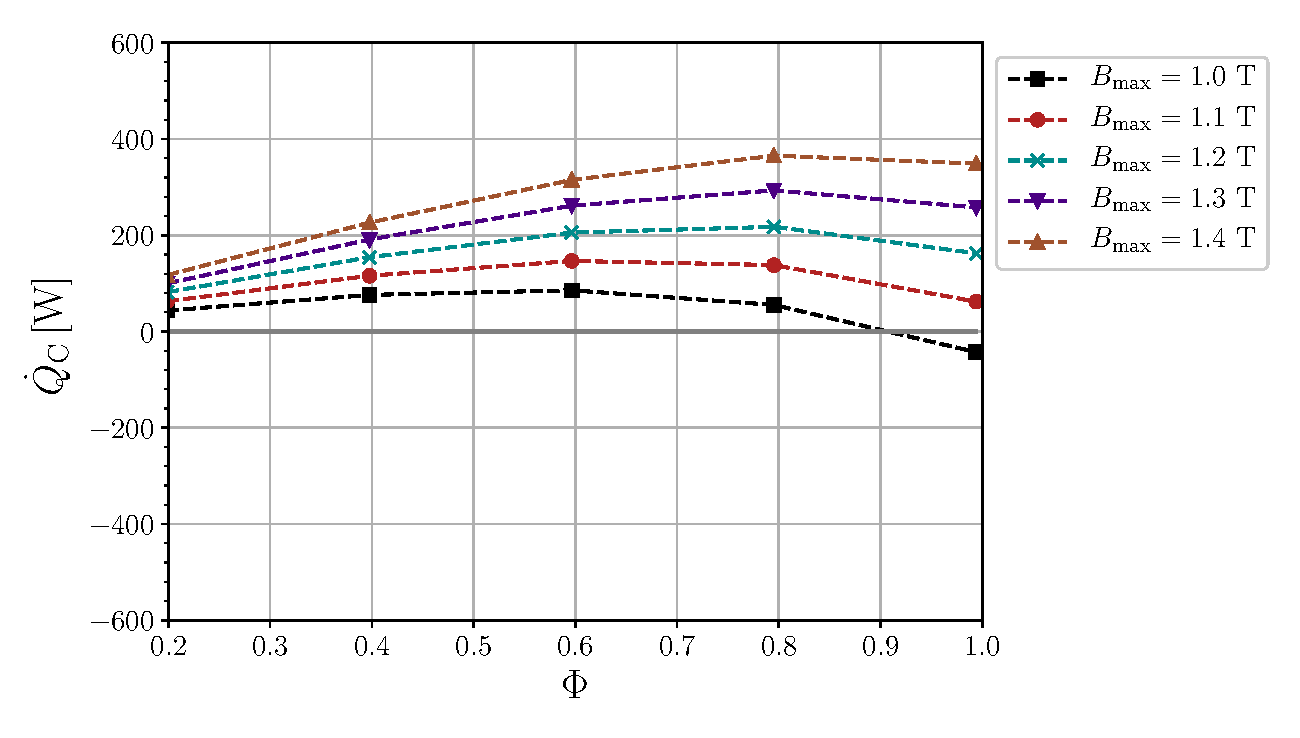
\includegraphics[width=8cm]{Fig10a-Qc_Phi_inst_f_1_Hmin_005_FB_100}\label{fig:Qc_phi_inst_1}}
\,
  \subfloat[$f = \SI{2}{\hertz}$]{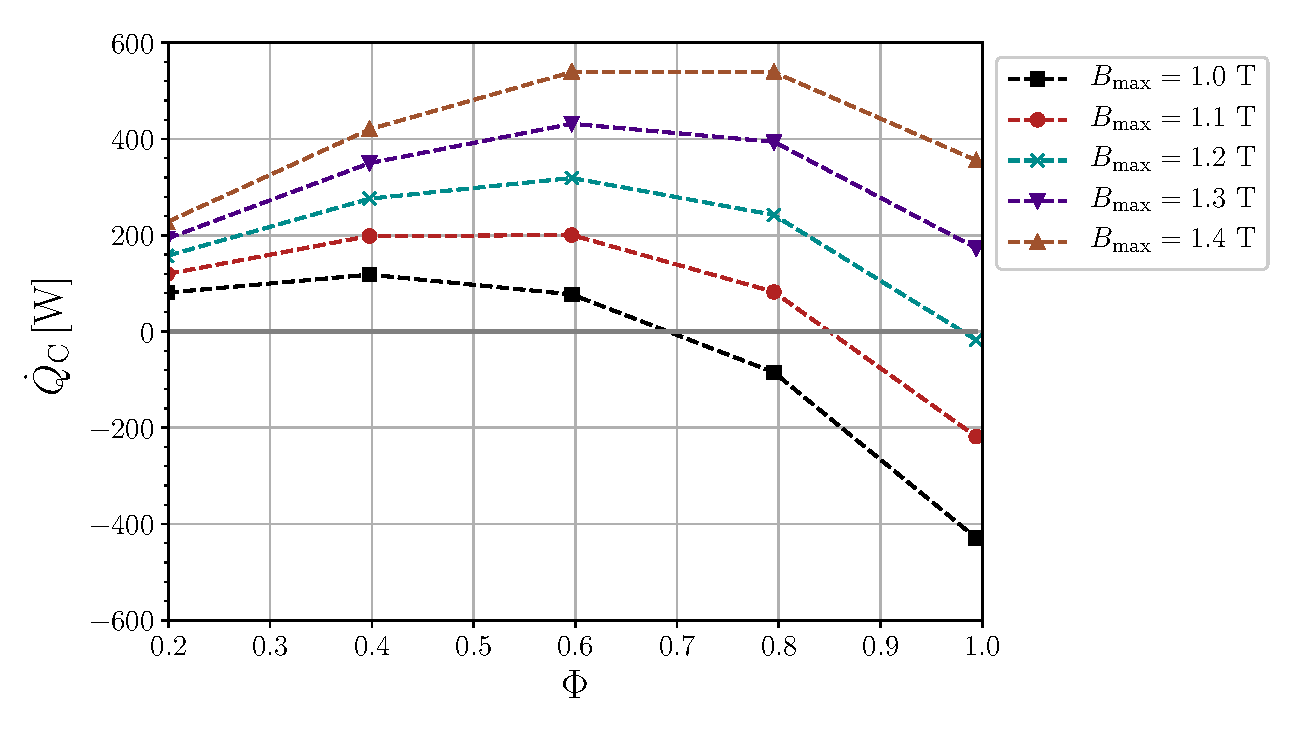
\includegraphics[width=8cm]{Fig10b-Qc_Phi_inst_f_2_Hmin_005_FB_100}\label{fig:Qc_phi_inst_2}}
  \caption{Cooling capacity as a function of utilization, for various values of the high magnetic field  for the instantaneous profile}
  \label{fig:qc_phi_inst}
\end{figure}

\begin{figure}[!ht]
  \centering
  \subfloat[Cooling capacity]{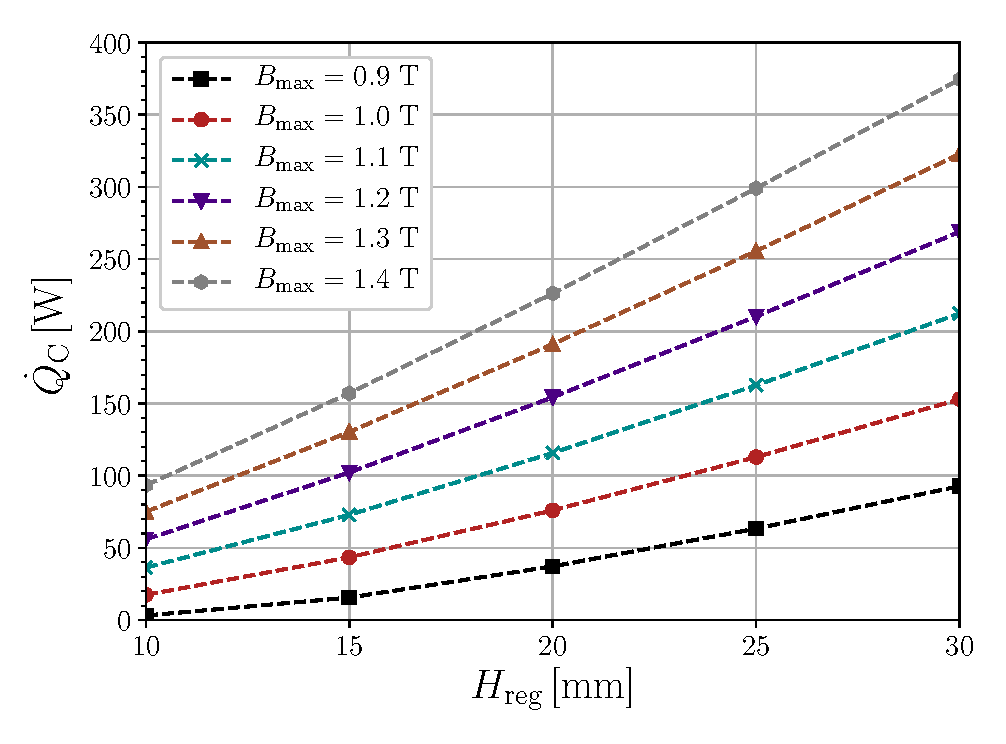
\includegraphics[width=9cm]{Fig11a-Qc_H_inst_f_1_Phi_40}\label{fig:Qc_H_inst_f_1_Phi_40}}
\quad
  \subfloat[Coefficient of performance]{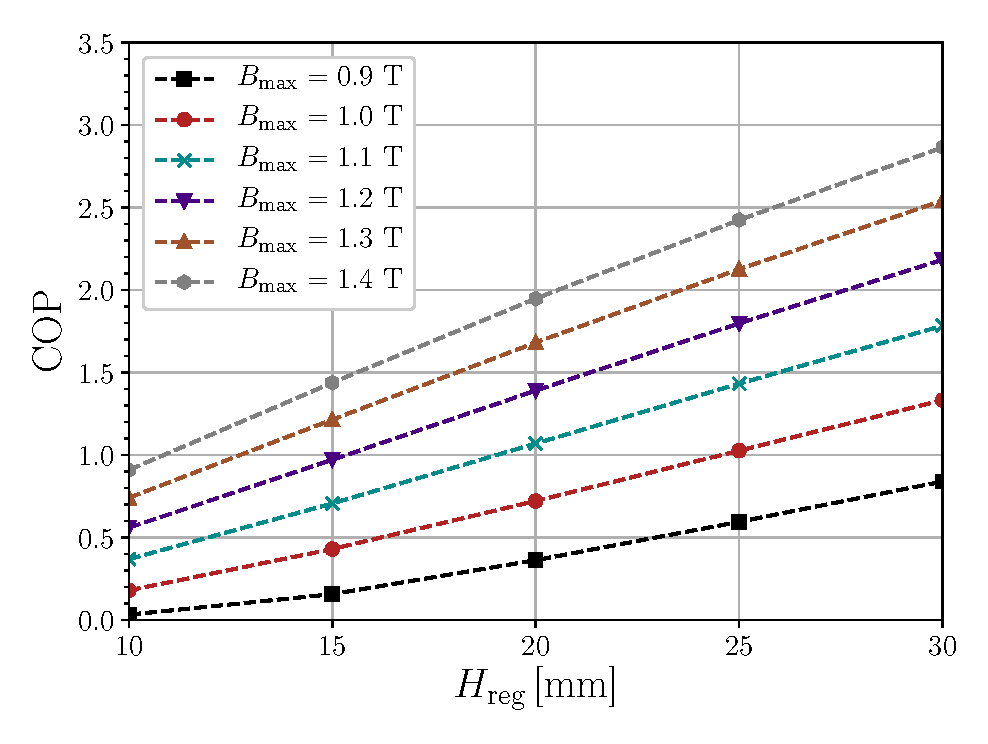
\includegraphics[width=9cm]{Fig11b-COP_H_inst_f_1_Phi_40}\label{fig:COP_H_inst_f_1_Phi_40}}
  \caption{Performance metrics as a function of the regenerator height (all other parameters were set as in Table~\ref{tab:params-cobem}, for utilization factor of 0.4) for various values of the high magnetic field of the instantaneous profile}
\label{fig:Qc_H_inst}
\end{figure}


The geometric parameters in \autoref{tab:params-cobem} were chosen from preliminary simulations, so they are not  optimal. To understand the impact of the regenerator geometry on the system performance with the instantaneous profile, the regenerator height was varied in Fig.~\ref{fig:Qc_H_inst}, and all other parameters from \autoref{tab:params-cobem} were kept fixed and with $\phi=0.4$. As expected, higher magnetic fields allow for smaller regenerators (hence more compact systems) to achieve a desired cooling capacity. For instance, to achieve a capacity of \SI{100}{\watt}, increasing the field from \num{1.0} to \SI{1.2}{\tesla} results in regenerators that are \SI{36}{\percent} smaller. Comparing the results for the cooling capacity and coefficient of performance, the trends are largely the same, as the former is more sensitive to variations in the magnetic field and regenerator height than the components of power.


\subsection{In-depth analysis of the  magnetic \textcolor{black}{ramp} profile}
\label{sec:performance-an-amr-1}

Based on the better performance of the instantaneous profile, the ramp profile is a naturally suitable target profile for the design of magnetic refrigerators, and will be analyzed in this section, representing the second stage in the analysis of magnetic profiles.

Moving towards a more realistic model, casing losses are included, using the model from \cite{bib:trevizoli16_perfor_model}. The bed is enclosed in a solid casing of thickness $h\ped{csg}$, and two air layers of thickness $h\ped{air}$ separate the AMR and its casing from the inner and outer magnet cylinders, as shown in \autoref{fig:amr-casing}. The optimal design of such magnetic cylinders aiming at a particular magnetic profile  will be the subject of future publications. 

\begin{figure}[!ht]
  \centering
  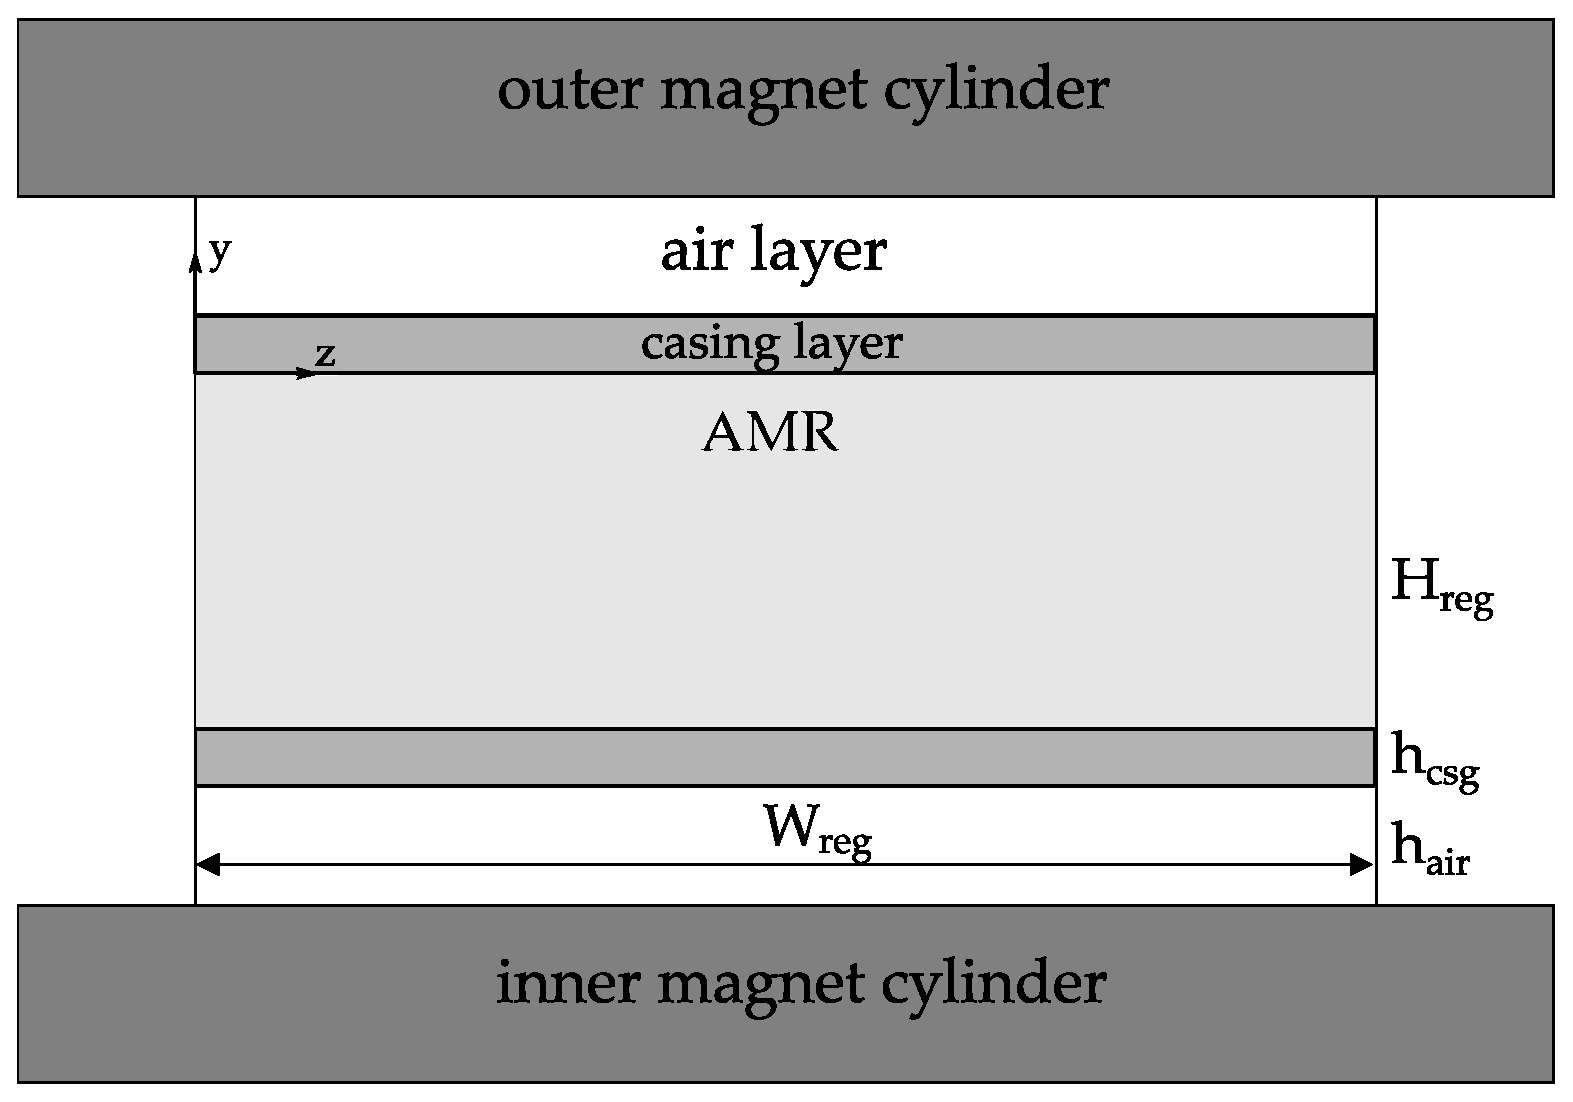
\includegraphics[width=7cm]{Fig12-amr-casing}
  \caption{Model for the casing losses in regenerators}
  \label{fig:amr-casing}
\end{figure}

\nomenclature[ia]{air}{air layer between magnets and regenerators}
\nomenclature[ah]{$h$}{thickness [\si{\meter}]}

Preliminary analyses carried out by \cite{bib:peixer17-perfor-amrs} showed that a stainless steel casing with a thickness of $h\ped{csg} = \SI{0.5}{\mm}$ is thick enough to ensure mechanical integrity and easy manufacturing, while being thin enough to accommodate the material with a low thermal conductivity.

In addition, in the present study, an air gap clearance thickness was set at $h\ped{air} = \SI{1}{\mm}$. This value gave rise to a peak in cooling capacity due to the compromise between minimizing losses and maximizing the magnetocaloric mass.  The thermophysical properties of stainless steel and air were also obtained with interpolation of tables exported by the EES software \cite{bib:klein13-ees}.

The simulations in this section also use multilayer regenerators. A summary of all parameters adopted in this section, including the Curie temperatures and volumetric fractions (relative to the length of the bed) of each layer is presented in \autoref{tab:params-ramp}. In addition, in the following results, Type S valves are used, with valve power calculated by \autoref{eq:198}.

\begin{table}[!ht]
  \centering
  \begin{tabular}{c|c}
\hline
    \textbf{Parameter} & \textbf{Value} \\
\hline
$W\ped{reg}$ & \SI{30}{\mm} \\
$L\ped{reg}$ & \SI{85}{\mm} \\
$N\ped{reg}$ & \num{8} \\
$N\ped{valve}$ & \num{16} \\
$f$ & \SI{1}{\hertz} \\
$T\ped{H}$ & \SI{305.5}{\kelvin} = \SI{32.5}{\celsius} \\
$\tc$ & \SI{270.5}{\kelvin} = \SI{-2.5}{\celsius} \\
$D\ped{p}$ & \SI{350}{\micro\meter} \\
$h\ped{csg}$ & \SI{0.5}{\mm} \\
$h\ped{air}$ & \SI{1}{\mm} \\
Casing material & Stainless steel \\
Number of layers & \num{3} \\
Curie temperatures of each layer & \num{273}, \num{283}, \SI{290}{\kelvin} \\ 
Length fractions of each layer & \num{20}, \num{20}, \SI{60}{\percent}\\
\hline
  \end{tabular}
  \caption{Fixed parameters for the AMR simulations used in this chapter}
  \label{tab:params-ramp}
\end{table}

 Figure~\ref{fig:ramp-inst} shows the two profiles that will be used in this section and how they are synchronized. Regarding the magnetic profile, the magnitude of the high value will be varied to investigate the performance of the AMR system, while the minimum will be kept at $\bmin = \SI{0.05}{\tesla}$. 

\begin{figure}[!ht]
  \centering
  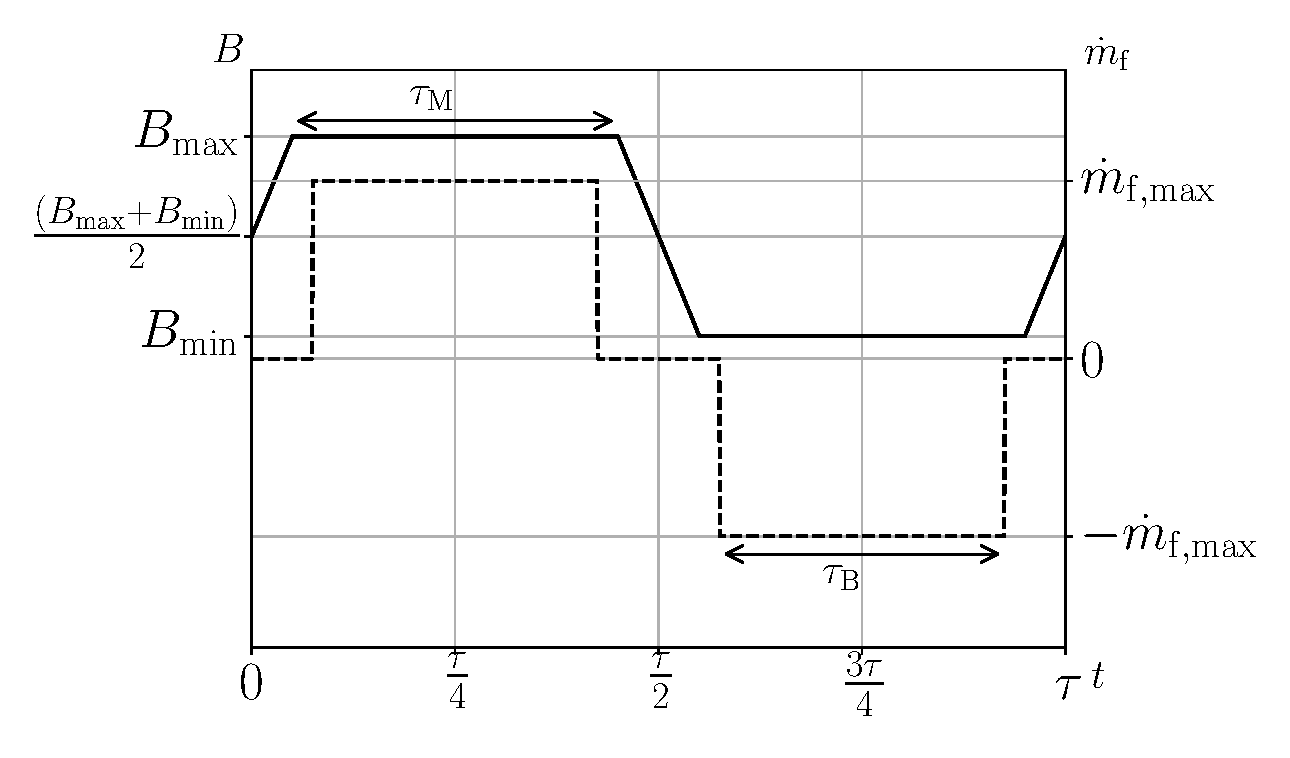
\includegraphics[width=7cm]{Fig13-profiles_rm_and_flow_instantaneous}
  \caption{Comparison between the magnetic \textcolor{black}{ramp} profile (solid line) and the instantaneous fluid flow profile (dashed line)}
  \label{fig:ramp-inst}
\end{figure}
 
\subsubsection{Performance curves for variable blow and magnetization fractions}
\label{sec:perf-curv-vary}

Figure~\ref{fig:Qc_COP_curves_phi40} shows the cooling capacity and coefficient of performance of the AMR system for a fixed utilization factor of \num{0.4} and for a magnetic profile with a maximum at \SI{1.3}{\tesla}, for variable blow and magnetization fractions. To facilitate the analysis, the results are plotted in terms of the ratio $\nicefrac{F\ped{M}}{F\ped{B}}$, with curves for different values of $F\ped{B}$. It is clear that both the cooling capacity and the coefficient of performance exhibit a peak at $F\ped{M} = F\ped{B}$. Moreover, to the right of the peak, i.e., for higher values of $F\ped{M}$, the reduction of both performance metrics is slower, meaning it is better to have a magnetization plateau that is wider than the fluid flow plateau.

The reduction in performance for $F\ped{M} > F\ped{B}$ can be explained by an increase in heat leakage through the casing, as the solid begins to lose energy to the environment when the fluid is not flowing. For $F\ped{M} < F\ped{B}$,  the fluid begins to flow when the solid is not totally warmed up, losing effectiveness.

\begin{figure}[!ht]
  \centering
  \subfloat[Cooling capacity]{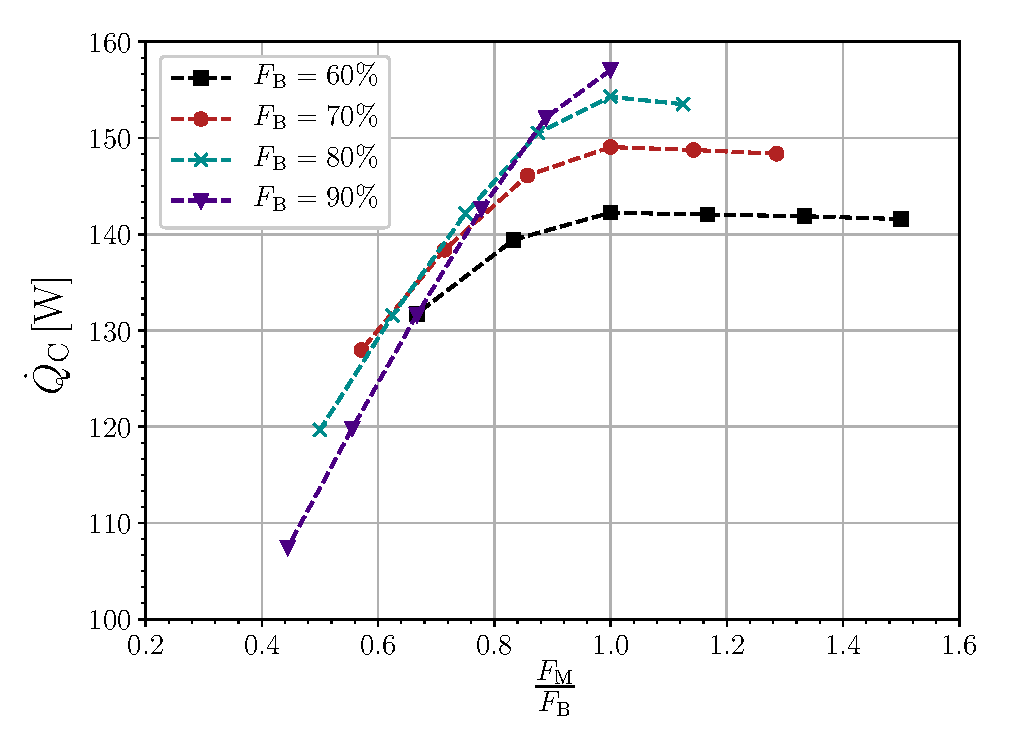
\includegraphics[width=5cm]{Fig14a-Qc_FM_ramp_f_1_Phi_40_35K_1300mT}\label{fig:Qc_FM_ramp_f_1_Phi_40_35K_1.3T}}
\quad
 \subfloat[Coefficient of performance]{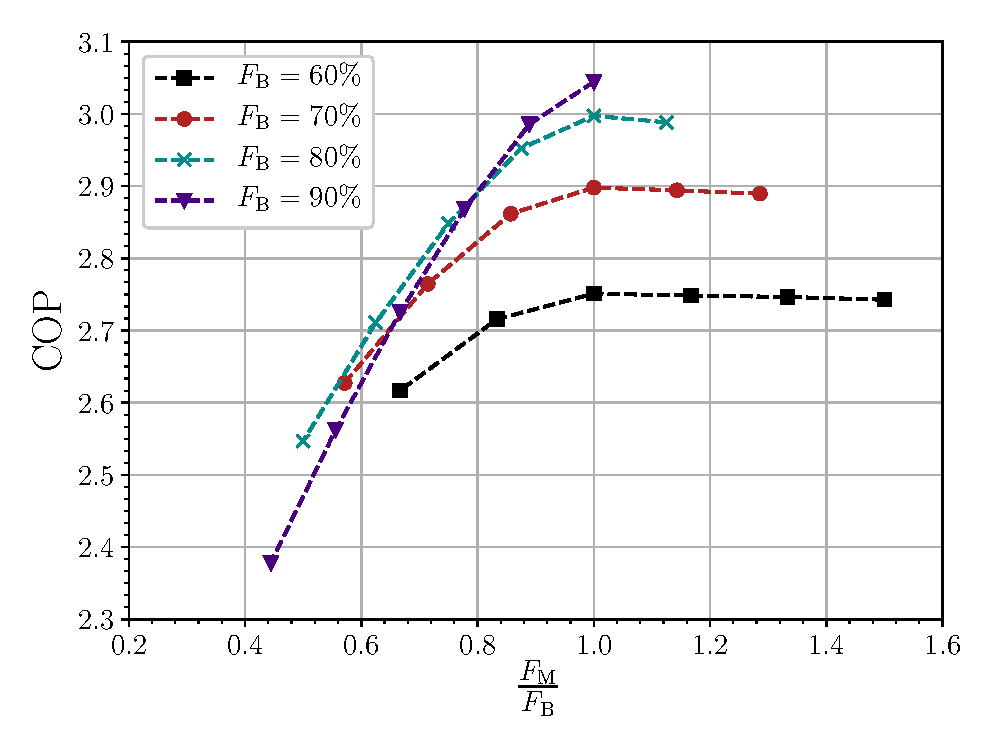
\includegraphics[width=5cm]{Fig14b-COP_FM_ramp_f_1_Phi_40_35K_1300mT}\label{fig:COP_FM_ramp_f_1_Phi_40_35K_1.3T}}
  \caption{Performance of the AMR system for various blow and magnetization fractions, utilization of 0.4 and and high magnetic field of \SI{1.3}{\tesla}}
  \label{fig:Qc_COP_curves_phi40}
\end{figure}

The influence of the utilization is demonstrated in \autoref{fig:Qc_curves_ramp_phi}, where the cooling capacity is plotted for different utilization factors. For increasing $\Phi$ in this range, not only do the overall values of cooling capacity increase, but also the importance of choosing the blow fraction becomes clearer. In these ranges of utilization and blow fraction,  the cooling capacity increases because the higher transfer rate associated with higher flow rates dominates over the loss of regenerator effectiveness.

\begin{figure}[!ht]
  \centering
  \subfloat[$\Phi = \num{0.2}$]{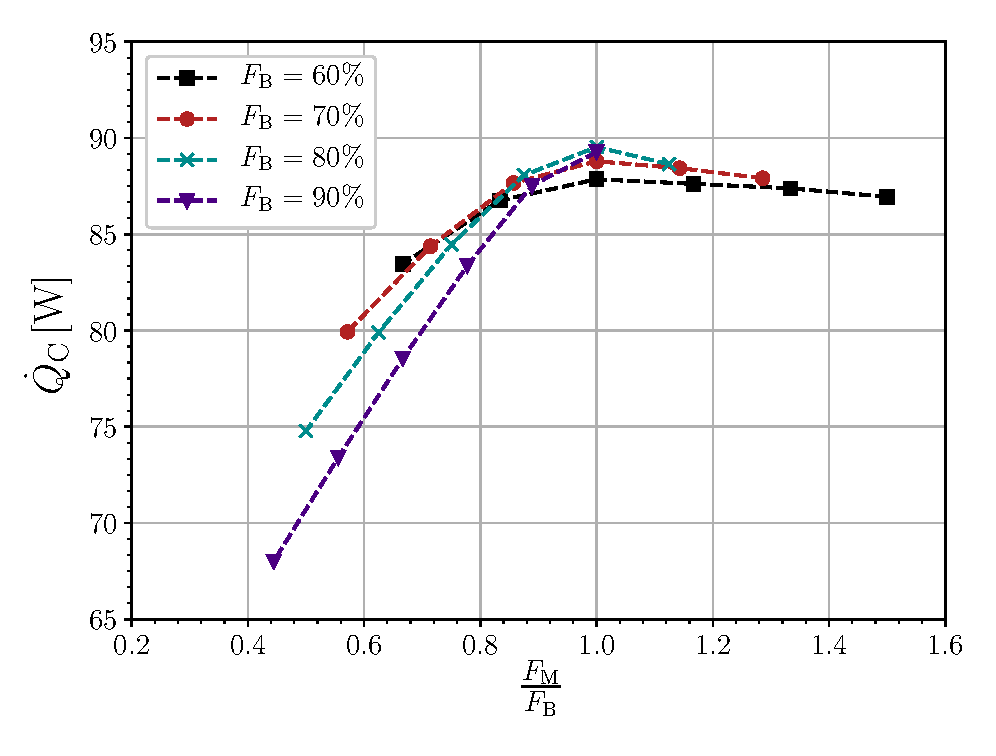
\includegraphics[width=5cm]{Fig15a-Qc_FM_ramp_f_1_Phi_20_35K_1300mT}\label{fig:Qc_FM_ramp_f_1_Phi_20_35K_1.3T}}
\quad
 \subfloat[$\Phi = \num{
0.5}$]{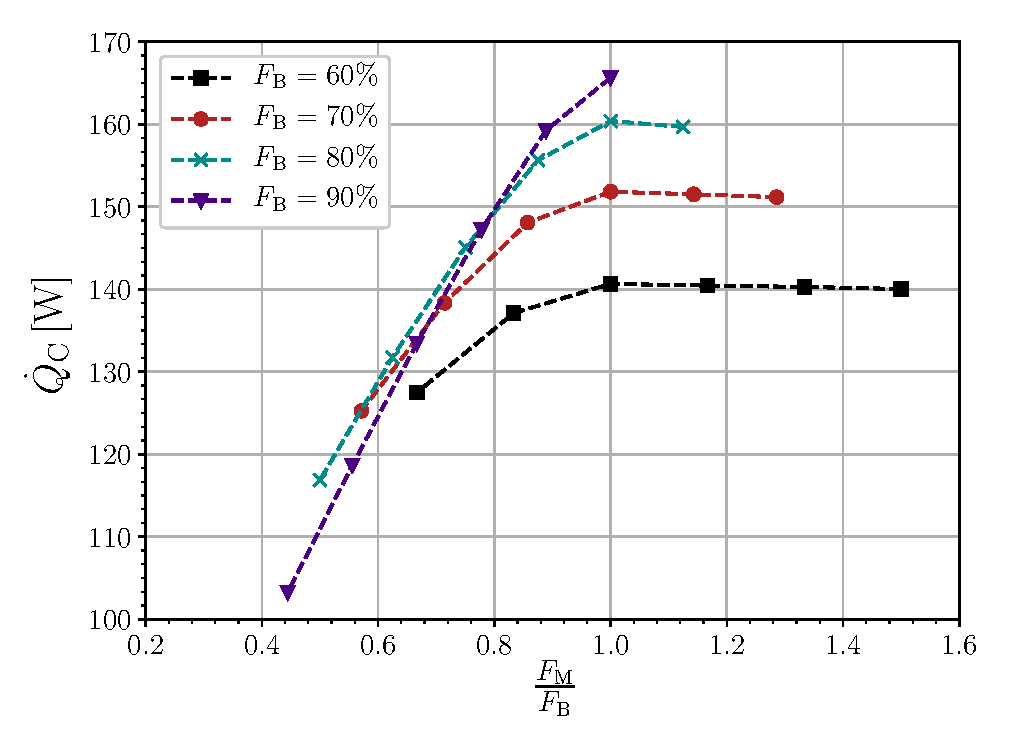
\includegraphics[width=5cm]{Fig15b-Qc_FM_ramp_f_1_Phi_50_35K_1300mT}\label{fig:COP_FM_ramp_f_1_Phi_50_35K_1.3T}}
  \caption{Influence of utilization on the cooling capacity of the AMR system for  various blow and magnetization fractions, with high magnetic field of \SI{1.3}{\tesla}}
  \label{fig:Qc_curves_ramp_phi}
\end{figure}

The above results can be evaluated from another point of view with \autoref{fig:COP_maps_ramp_FM}, where the coefficient of performance is plotted as contour levels. This type of map is useful because, since $\bmin$ and $\tau$ are fixed, each point in this graph completely characterizes a magnetic ramp profile, and each subplot with fixed $\Phi$ and $F\ped{B}$ characterizes the fluid flow profile. As expected, the performance increases for the higher values both $\bmax$ and $F\ped{M}$, where the  magnetic ramp profile tends to the instantaneous magnetic profile with a large amplitude. Confirming the previous trends, the results are less sensitive to the magnetization fraction when $F\ped{M} \ge F\ped{B}$. 

\begin{figure}[!ht]
  \centering
  \subfloat[$\Phi = 0.2, F\ped{B} = \SI{60}{\percent}$]{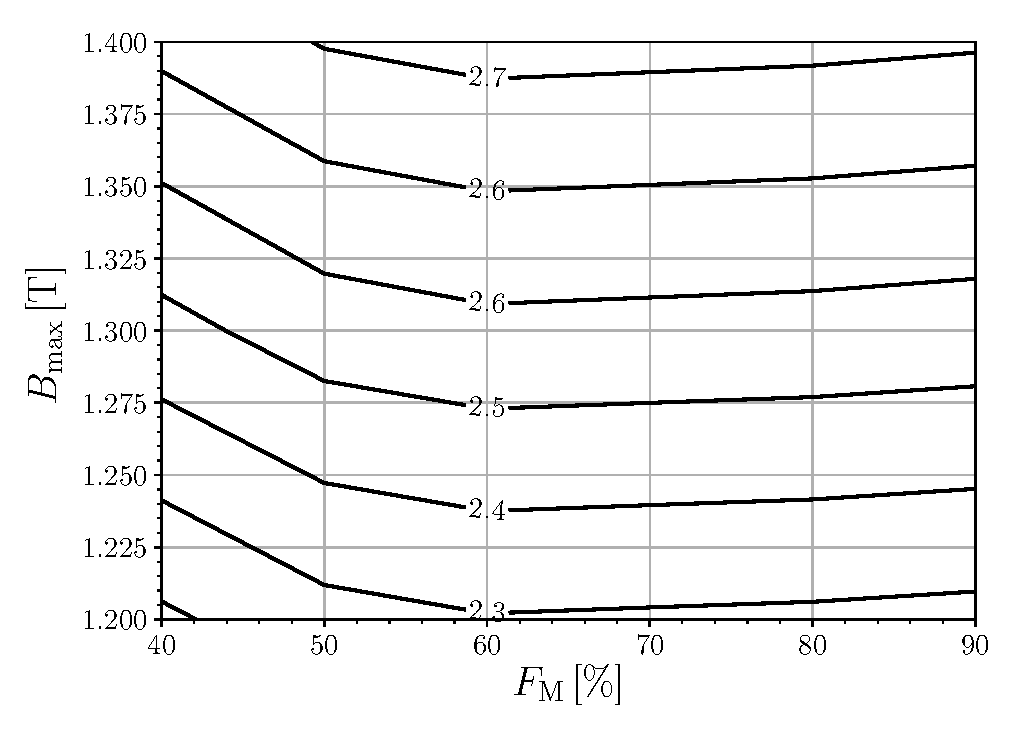
\includegraphics[width=5cm]{Fig16a-COP_ramp_map_f_1_Phi_20_FB_60_35K_Valv_ASCO}\label{fig:COP_ramp_map_f_1_Phi_20_FB_70_35K_Valv_ASCO}}
\quad
 \subfloat[$\Phi= 0.2, F\ped{B} = \SI{90}{\percent}$]{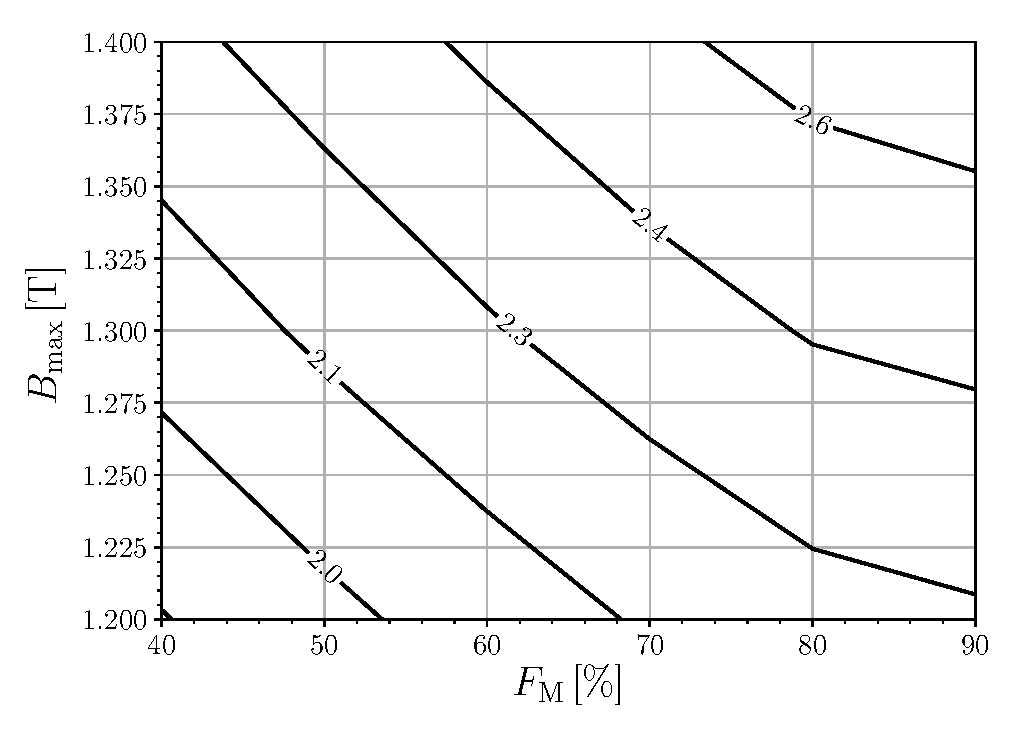
\includegraphics[width=5cm]{Fig16b-COP_ramp_map_f_1_Phi_20_FB_90_35K_Valv_ASCO}\label{fig:COP_ramp_map_f_1_Phi_20_FB_90_35K_Valv_ASCO}} \\
  \subfloat[$\Phi = 0.4, F\ped{B} = \SI{60}{\percent}$]{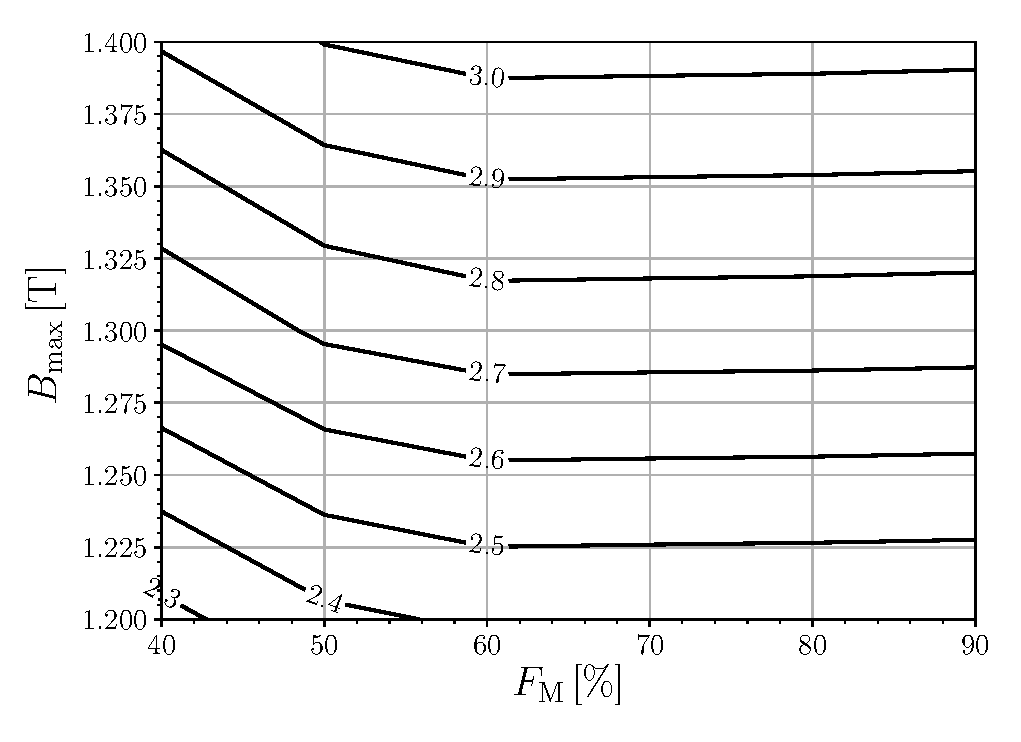
\includegraphics[width=5cm]{Fig16c-COP_ramp_map_f_1_Phi_40_FB_60_35K_Valv_ASCO}\label{fig:COP_ramp_map_f_1_Phi_60_FB_90_35K_Valv_ASCO}}
\quad
 \subfloat[$\Phi = 0.4, F\ped{B} = \SI{90}{\percent}$]{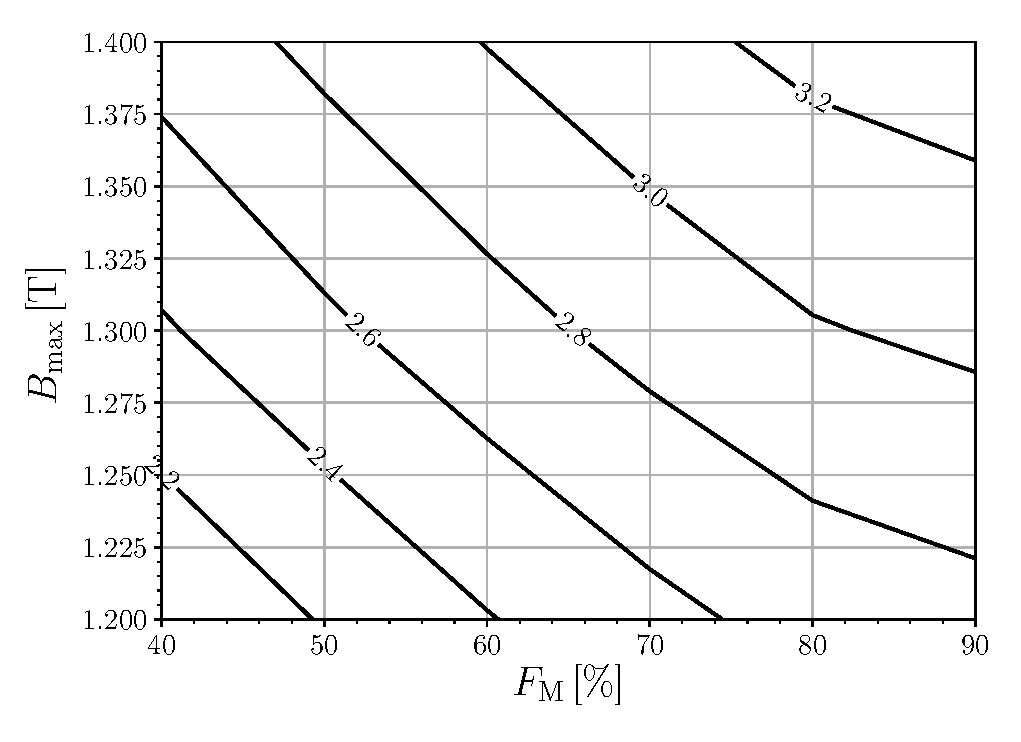
\includegraphics[width=5cm]{Fig16d-COP_ramp_map_f_1_Phi_40_FB_90_35K_Valv_ASCO}\label{fig:COP_ramp_map_f_1_Phi_40_FB_90_35K_Valv_ASCO}}
  \caption{Influence of utilization and blow fraction on the coefficient of performance of the AMR system for varying high magnetic field and magnetization fraction}
  \label{fig:COP_maps_ramp_FM}
\end{figure}

\subsubsection{Geometric analysis of the regenerators using the magnetic ramp profile}
\label{sec:geom-analys-regen}

All previous results assumed a fixed regenerator geometry, with the goal of identifying the optimal fluid and magnetic profile parameters. It became clear that the magnetization fraction should be as large as possible, but that raises some challenges in realizing abrupt changes in the magnetic field. The value of $F\ped{M} = \SI{70}{\percent}$ is then chosen as a compromise, with a corresponding $F\ped{B} = F\ped{M}$. The mean value of the utilization factor of $\Phi = 0.4$ is also chosen as reference in the next results.

Figure~\ref{fig:qc-cop-eta-amr-height} shows the cooling capacity, coefficient of performance and second-law efficiency for varying magnetic field and regenerator height. As expected, larger regenerators can produce the desired performance with lower magnetic fields. It can also be seen that this configuration for an AMR system can achieve values of $\etasec$ compatible with conventional vapor compression systems \cite{HERMES20081341,NEGRAO20113051}, although these numerical results do not include mechanical losses.

\begin{figure}[!ht]
  \centering
\subfloat[Cooling capacity (solid lines) and coefficient of performance (dashed lines)]{  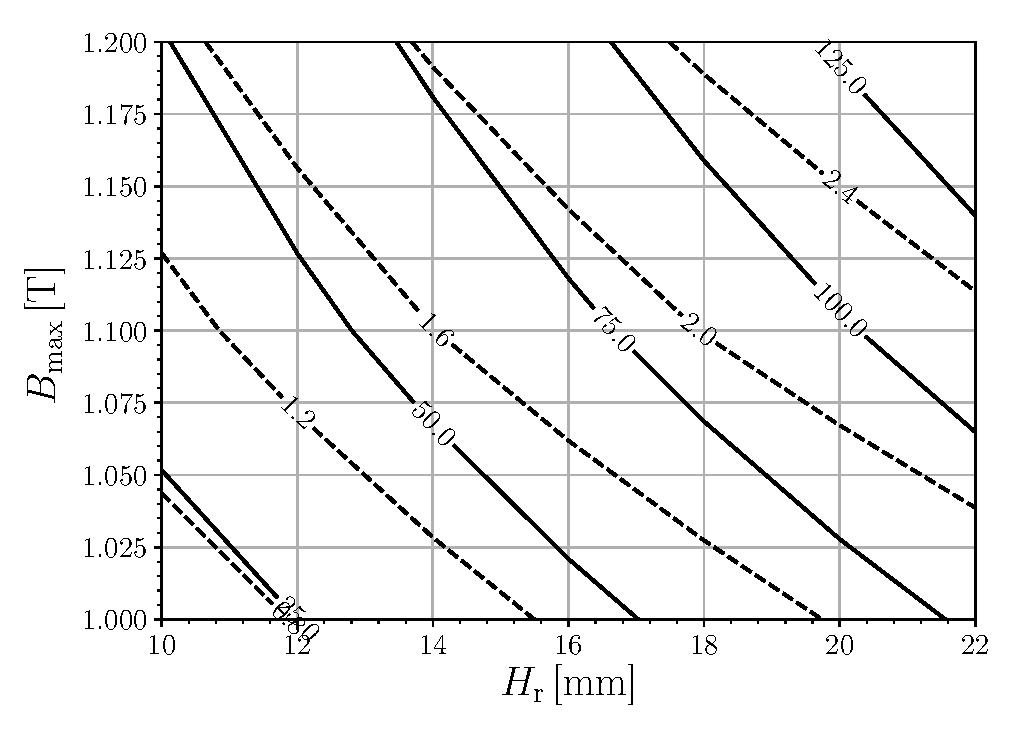
\includegraphics[width=5cm]{Fig17a-Qc_COP_combined_H_regW30}\label{fig:Qc_COP_Hreg}}
\,
\subfloat[Second-law efficiency]{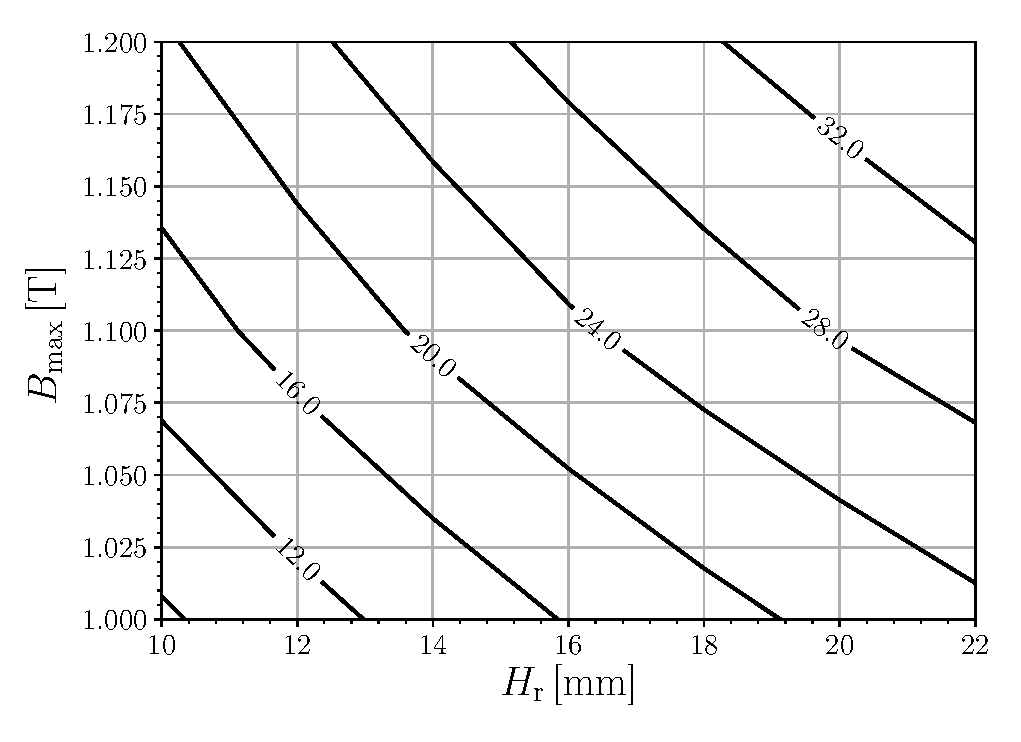
\includegraphics[width=5cm]{Fig17b-eta_H_regW30}\label{fig:eta_Hreg}}
  \caption{Performance of the AMR with varying regenerator height and high magnetic field, with fixed $F\ped{M} = F\ped{B} = \SI{70}{\percent}$ and $\Phi = 0.4$}
  \label{fig:qc-cop-eta-amr-height}
\end{figure}


\section{Conclusions}
\label{sec:final-considerations}

To the authors' knowledge, this is the first study where magnetic and fluid flow profiles for an AMR model are mathematically modeled and the model parameters are changed in an integrated and systematic  way. The instantaneous (square wave), rectified cosine and ramp magnetic profiles were implemented in an AMR model, together with an instantaneous fluid flow profile, and the profile parameters were varied simultaneously with the regenerator geometric parameters. These waveforms can be found in existing MR devices published in the literature. A valve model was also incorporated into a more realistic computation of the coefficient of performance.

When comparing the instantaneous  and the rectified cosing magnetic profiles, the cooling capacity associated with the former can be almost \SI{200}{\percent} higher than with the latter, for the same utilization and average high magnetic field and considering optimal blow fractions. The rectified cosing profile suffers from high values of the low magnetic field, and reduction of blow fraction up to the minimum tested value of \SI{60}{\percent} is not enough to overcome the loss in cooling capacity resulting from this effect. 

An analysis of power contributions showed that the cost of the higher cooling capacity for the instantaneous profile is a higher valve power associated with the longer blow duration, dominating the other contributions. However, the coefficient of performance is still higher for the square wave. Hence, even though sinusoidal waveforms can be obtained with more compact systems, step-like variations of high amplitude of the magnetic field are preferred if performance is more critical.

The ramp magnetic profile is a feasible approximation for the instantaneous profile without abrupt changes in the magnetic field plateaus. For an AMR device operating with this  profile and the instantaneous fluid flow profile, both cooling capacity and coefficient of performance are maximized if the blow duration is equal to the period of constant magnetic field; if this exact synchronization is not possible, making the magnetization plateau wider than the flow plateau results in smaller reduction of the performance metrics than if it is narrower. 

With this strategy and using average values of utilization, it is possible to achieve second-law efficiency levels compatible with vapor-compression systems. Hence the ramp magnetic profile is identified as a suitable target profile in the design of magnetic circuits for AMR devices.

\section*{Supplementary Material}
\label{sec:suppl-mater}

The datasets for the results shown in this paper, the source code used to produce the figures and the \LaTeX{} manuscript for this work are available at \cite{bib:fortkamp19-repo-pprof}.

\section*{Conflict of Interest Statement}

There is no actual or potential conflict of interest including any financial, personal or other relationships with other people or organizations that could inappropriately influence, or be perceived to influence, the present work.

\acknowledgement{This work was funded by the Brazilian Federal Government (CAPES PTI program, Process no. 88887.194773/2018-00, CNPq Grant no. 443696/2014-4 and EMBRAPII) and by the State of Santa Catarina (FAPESC/INCT). The authors acknowledge the continuous support from Embraco.
}


% BibTeX users please use one of
%\bibliographystyle{spbasic}      % basic style, author-year citations
%\bibliographystyle{spmpsci}      % mathematics and physical sciences
\bibliographystyle{unsrtnat}
%\renewcommand{\refname}{}
%\bibliographystyle{spphys}       % APS-like style for physics

\bibliography{Thermo-Foam-Ref,thesis}

\end{document}             

%%% Local Variables:
%%% mode: latex
%%% TeX-master: t
%%% End:
